\documentclass[10pt,a4paper,twocolumn]{article}
\usepackage{fontspec}
\usepackage[margin=0.62in,columnsep=0.25in]{geometry}
\usepackage{titlesec}
\usepackage{graphicx}
\usepackage{booktabs}
\usepackage{array}
\usepackage{tabularx}
\usepackage{xcolor}
\usepackage{amsmath}
\usepackage{amssymb}
\usepackage{enumitem}
\usepackage{caption}
\usepackage{float}
\usepackage[hidelinks]{hyperref}
\usepackage{fancyhdr}

\setmainfont{texgyretermes}[Extension=.otf, UprightFont=*-regular, BoldFont=*-bold, ItalicFont=*-italic, BoldItalicFont=*-bolditalic]
\newfontfamily\devanagarifont[Path=./fonts/, Scale=0.92, Script=Devanagari]{NotoSansDevanagari-Regular.ttf}
\newcommand{\dn}[1]{{\devanagarifont #1}}
% generated by make_numbers.py - do not edit
\newcommand{\AblUnEnt}{38.3}
\newcommand{\AblValEM}{38.0}
\newcommand{\AblValLoss}{0.483}
\newcommand{\AccBaseSeen}{\textcolor{red}{??}}
\newcommand{\AccBaseUnEnt}{\textcolor{red}{??}}
\newcommand{\AccBaseUnWord}{\textcolor{red}{??}}
\newcommand{\AccBaseVal}{\textcolor{red}{??}}
\newcommand{\AccBestSeen}{63.5}
\newcommand{\AccBestUnEnt}{63.1}
\newcommand{\AccBestUnWord}{45.3}
\newcommand{\AccBestVal}{65.6}
\newcommand{\AccDpoHighSeen}{69.4}
\newcommand{\AccDpoHighUnEnt}{62.4}
\newcommand{\AccDpoHighUnWord}{42.8}
\newcommand{\AccDpoHighVal}{63.0}
\newcommand{\AccDpoLowSeen}{39.4}
\newcommand{\AccDpoLowUnEnt}{31.9}
\newcommand{\AccDpoLowUnWord}{32.5}
\newcommand{\AccDpoLowVal}{35.4}
\newcommand{\AccFullSeen}{83.9}
\newcommand{\AccFullUnEnt}{81.0}
\newcommand{\AccFullUnWord}{45.3}
\newcommand{\AccFullVal}{82.9}
\newcommand{\AccLoraFourSeen}{60.9}
\newcommand{\AccLoraFourUnEnt}{55.8}
\newcommand{\AccLoraFourUnWord}{44.3}
\newcommand{\AccLoraFourVal}{54.1}
\newcommand{\AccLoraOneSeen}{32.2}
\newcommand{\AccLoraOneUnEnt}{36.4}
\newcommand{\AccLoraOneUnWord}{31.3}
\newcommand{\AccLoraOneVal}{36.0}
\newcommand{\AccLoraSixteenSeen}{63.5}
\newcommand{\AccLoraSixteenUnEnt}{63.1}
\newcommand{\AccLoraSixteenUnWord}{45.3}
\newcommand{\AccLoraSixteenVal}{65.6}
\newcommand{\AdaAccBestSeen}{80.8}
\newcommand{\AdaAccBestUnEnt}{80.9}
\newcommand{\AdaAccBestUnWord}{56.4}
\newcommand{\AdaAccBestVal}{80.2}
\newcommand{\AdaAccFourSeen}{48.7$\pm$5.1}
\newcommand{\AdaAccFourUnEnt}{51.9$\pm$1.2}
\newcommand{\AdaAccFourUnWord}{36.1$\pm$2.6}
\newcommand{\AdaAccFourVal}{50.2$\pm$3.0}
\newcommand{\AdaAccFullSeen}{83.9}
\newcommand{\AdaAccFullUnEnt}{81.0}
\newcommand{\AdaAccFullUnWord}{45.3}
\newcommand{\AdaAccFullVal}{82.9}
\newcommand{\AdaAccOneSeen}{37.1$\pm$4.2}
\newcommand{\AdaAccOneUnEnt}{35.5$\pm$2.4}
\newcommand{\AdaAccOneUnWord}{31.5$\pm$3.0}
\newcommand{\AdaAccOneVal}{35.8$\pm$1.8}
\newcommand{\AdaAccSixteenSeen}{78.0$\pm$4.6}
\newcommand{\AdaAccSixteenUnEnt}{76.9$\pm$5.9}
\newcommand{\AdaAccSixteenUnWord}{51.4$\pm$6.2}
\newcommand{\AdaAccSixteenVal}{77.6$\pm$3.7}
\newcommand{\AdaBest}{LoRA $r=16$, seed 43}
\newcommand{\AdaBestRank}{16}
\newcommand{\AdaBestSeed}{43}
\newcommand{\AdaChainFourSeen}{32.1$\pm$3.7}
\newcommand{\AdaChainFourUnEnt}{32.2$\pm$6.5}
\newcommand{\AdaChainFourUnWord}{3.5$\pm$1.7}
\newcommand{\AdaChainFourVal}{29.7$\pm$5.0}
\newcommand{\AdaChainFullSeen}{81.6}
\newcommand{\AdaChainFullUnEnt}{72.9}
\newcommand{\AdaChainFullUnWord}{3.1}
\newcommand{\AdaChainFullVal}{74.5}
\newcommand{\AdaChainOneSeen}{2.9$\pm$1.5}
\newcommand{\AdaChainOneUnEnt}{3.0$\pm$1.6}
\newcommand{\AdaChainOneUnWord}{0.4$\pm$0.7}
\newcommand{\AdaChainOneVal}{2.0$\pm$0.6}
\newcommand{\AdaChainSixteenSeen}{70.8$\pm$4.6}
\newcommand{\AdaChainSixteenUnEnt}{66.1$\pm$5.2}
\newcommand{\AdaChainSixteenUnWord}{8.8$\pm$3.7}
\newcommand{\AdaChainSixteenVal}{67.5$\pm$4.4}
\newcommand{\AdaDpoHighAnsSeen}{99$\pm$0}
\newcommand{\AdaDpoHighAnsUnEnt}{98$\pm$0}
\newcommand{\AdaDpoHighAnsUnWord}{85$\pm$1}
\newcommand{\AdaDpoHighAnsVal}{99$\pm$0}
\newcommand{\AdaDpoHighLr}{3e-5}
\newcommand{\AdaDpoHighPpl}{61.34$\pm$0.01}
\newcommand{\AdaDpoHighPplFull}{53.79$\pm$0.00}
\newcommand{\AdaDpoHighSeen}{82.3$\pm$0.7}
\newcommand{\AdaDpoHighStep}{500}
\newcommand{\AdaDpoHighStepZero}{0.693147/0.693147/0.693147}
\newcommand{\AdaDpoHighUnEnt}{81.0$\pm$0.8}
\newcommand{\AdaDpoHighUnWord}{49.0$\pm$1.4}
\newcommand{\AdaDpoHighVal}{81.2$\pm$0.3}
\newcommand{\AdaDpoLowAnsSeen}{100$\pm$0}
\newcommand{\AdaDpoLowAnsUnEnt}{100$\pm$0}
\newcommand{\AdaDpoLowAnsUnWord}{98$\pm$0}
\newcommand{\AdaDpoLowAnsVal}{100$\pm$0}
\newcommand{\AdaDpoLowLr}{1e-5}
\newcommand{\AdaDpoLowPpl}{61.30$\pm$0.00}
\newcommand{\AdaDpoLowPplFull}{53.76$\pm$0.00}
\newcommand{\AdaDpoLowSeen}{80.9$\pm$0.4}
\newcommand{\AdaDpoLowStep}{100}
\newcommand{\AdaDpoLowStepZero}{0.693147/0.693147/0.693147}
\newcommand{\AdaDpoLowUnEnt}{80.7$\pm$0.3}
\newcommand{\AdaDpoLowUnWord}{55.6$\pm$0.4}
\newcommand{\AdaDpoLowVal}{80.7$\pm$0.2}
\newcommand{\AdaFixHighAnsSeen}{97}
\newcommand{\AdaFixHighAnsUnEnt}{95}
\newcommand{\AdaFixHighAnsUnWord}{79}
\newcommand{\AdaFixHighAnsVal}{96}
\newcommand{\AdaFixHighPpl}{61.48}
\newcommand{\AdaFixHighPplFull}{53.87}
\newcommand{\AdaFixHighSeen}{81.5}
\newcommand{\AdaFixHighUnEnt}{79.7}
\newcommand{\AdaFixHighUnWord}{42.2}
\newcommand{\AdaFixHighVal}{79.3}
\newcommand{\AdaFixLowAnsSeen}{74}
\newcommand{\AdaFixLowAnsUnEnt}{72}
\newcommand{\AdaFixLowAnsUnWord}{60}
\newcommand{\AdaFixLowAnsVal}{69}
\newcommand{\AdaFixLowPpl}{61.96}
\newcommand{\AdaFixLowPplFull}{54.12}
\newcommand{\AdaFixLowSeen}{52.0}
\newcommand{\AdaFixLowUnEnt}{46.8}
\newcommand{\AdaFixLowUnWord}{29.3}
\newcommand{\AdaFixLowVal}{43.4}
\newcommand{\AdaLossFour}{0.151$\pm$0.016}
\newcommand{\AdaLossOne}{0.490$\pm$0.014}
\newcommand{\AdaLossSixteen}{0.075$\pm$0.003}
\newcommand{\AdaLrFour}{1e-3}
\newcommand{\AdaLrOne}{3e-4}
\newcommand{\AdaLrSixteen}{1e-3}
\newcommand{\AdaPplBest}{61.30}
\newcommand{\AdaPplFour}{60.65$\pm$0.06}
\newcommand{\AdaPplFull}{63.50}
\newcommand{\AdaPplFullBase}{49.28}
\newcommand{\AdaPplFullBest}{53.77}
\newcommand{\AdaPplFullFour}{52.89$\pm$0.21}
\newcommand{\AdaPplFullFull}{58.62}
\newcommand{\AdaPplFullOne}{52.46$\pm$0.11}
\newcommand{\AdaPplFullSixteen}{53.84$\pm$0.07}
\newcommand{\AdaPplOne}{60.58$\pm$0.26}
\newcommand{\AdaPplSixteen}{61.36$\pm$0.06}
\newcommand{\AdaStepZeroDev}{1.9e-9}
\newcommand{\AdaStepZeroRuns}{10}
\newcommand{\AfterFour}{0.77}
\newcommand{\AfterOne}{1.01}
\newcommand{\AfterSixteen}{0.82}
\newcommand{\AnsBaseSeen}{\textcolor{red}{??}}
\newcommand{\AnsBaseUnEnt}{\textcolor{red}{??}}
\newcommand{\AnsBaseUnWord}{\textcolor{red}{??}}
\newcommand{\AnsBaseVal}{\textcolor{red}{??}}
\newcommand{\AnsDpoHighSeen}{96}
\newcommand{\AnsDpoHighUnEnt}{96}
\newcommand{\AnsDpoHighUnWord}{83}
\newcommand{\AnsDpoHighVal}{95}
\newcommand{\AnsDpoLowSeen}{64}
\newcommand{\AnsDpoLowUnEnt}{59}
\newcommand{\AnsDpoLowUnWord}{69}
\newcommand{\AnsDpoLowVal}{62}
\newcommand{\AnsFullSeen}{100}
\newcommand{\AnsFullUnEnt}{100}
\newcommand{\AnsFullUnWord}{98}
\newcommand{\AnsFullVal}{100}
\newcommand{\AnsLoraFourSeen}{100}
\newcommand{\AnsLoraFourUnEnt}{100}
\newcommand{\AnsLoraFourUnWord}{100}
\newcommand{\AnsLoraFourVal}{100}
\newcommand{\AnsLoraOneSeen}{100}
\newcommand{\AnsLoraOneUnEnt}{99}
\newcommand{\AnsLoraOneUnWord}{100}
\newcommand{\AnsLoraOneVal}{99}
\newcommand{\AnsLoraSixteenSeen}{100}
\newcommand{\AnsLoraSixteenUnEnt}{100}
\newcommand{\AnsLoraSixteenUnWord}{94}
\newcommand{\AnsLoraSixteenVal}{100}
\newcommand{\BestEpFour}{5}
\newcommand{\BestEpOne}{3}
\newcommand{\BestEpSixteen}{5}
\newcommand{\BestRank}{16}
\newcommand{\CCotAll}{35.0}
\newcommand{\CCotMod}{20.0}
\newcommand{\CCotModN}{1/5}
\newcommand{\CCotStd}{40.0}
\newcommand{\CCotStdN}{6/15}
\newcommand{\CCotTmpl}{20}
\newcommand{\CCotTok}{446.9}
\newcommand{\CCotTokRatio}{95}
\newcommand{\CCotTrunc}{4}
\newcommand{\CDeva}{98.5}
\newcommand{\CDirectAll}{30.0}
\newcommand{\CDirectMod}{20.0}
\newcommand{\CDirectModN}{1/5}
\newcommand{\CDirectStd}{33.3}
\newcommand{\CDirectStdN}{5/15}
\newcommand{\CDirectTmpl}{20}
\newcommand{\CDirectTok}{4.7}
\newcommand{\CDirectTrunc}{0}
\newcommand{\CScAll}{50.0}
\newcommand{\CScAllMean}{51.7}
\newcommand{\CScAllSd}{2.9}
\newcommand{\CScMod}{0.0}
\newcommand{\CScModMean}{0.0}
\newcommand{\CScModN}{0/5}
\newcommand{\CScSeedsStd}{66.7 / 73.3 / 66.7}
\newcommand{\CScStd}{66.7}
\newcommand{\CScStdMean}{68.9}
\newcommand{\CScStdN}{10/15}
\newcommand{\CScStdSd}{3.8}
\newcommand{\CScTmpl}{40}
\newcommand{\CScTok}{1,881.8}
\newcommand{\CScTokMean}{1,837}
\newcommand{\CScTokRatio}{400}
\newcommand{\CScTokSample}{376.4}
\newcommand{\CScTrunc}{5}
\newcommand{\CTwoAgree}{50.0}
\newcommand{\CTwoAgreeAll}{50.0}
\newcommand{\CTwoAvgAgree}{56.7}
\newcommand{\CTwoAvgCot}{22}
\newcommand{\CTwoAvgKappa}{0.13}
\newcommand{\CTwoConsCot}{9}
\newcommand{\CTwoConsDirect}{1}
\newcommand{\CTwoConsistent}{10}
\newcommand{\CTwoFirst}{80.0}
\newcommand{\CTwoFirstN}{48}
\newcommand{\CTwoKappa}{0.14}
\newcommand{\CTwoLongRight}{15}
\newcommand{\CTwoLonger}{63.3}
\newcommand{\CTwoLongerN}{38}
\newcommand{\CTwoPairs}{30}
\newcommand{\CTwoPosBias}{66.7}
\newcommand{\CTwoPosBiasN}{20}
\newcommand{\CTwoProblems}{15}
\newcommand{\CTwoShortRight}{15}
\newcommand{\CTwoShortRightProblems}{M02, S01, S03, S05, S06, S07}
\newcommand{\CTwoTopAB}{55}
\newcommand{\ChainBaseSeen}{\textcolor{red}{??}}
\newcommand{\ChainBaseUnEnt}{\textcolor{red}{??}}
\newcommand{\ChainBaseUnWord}{\textcolor{red}{??}}
\newcommand{\ChainBaseVal}{\textcolor{red}{??}}
\newcommand{\ChainBestSeen}{56.0}
\newcommand{\ChainBestUnEnt}{53.5}
\newcommand{\ChainBestUnWord}{5.5}
\newcommand{\ChainBestVal}{54.8}
\newcommand{\ChainDpoHighSeen}{62.2}
\newcommand{\ChainDpoHighUnEnt}{52.0}
\newcommand{\ChainDpoHighUnWord}{5.0}
\newcommand{\ChainDpoHighVal}{53.0}
\newcommand{\ChainDpoLowSeen}{28.6}
\newcommand{\ChainDpoLowUnEnt}{22.3}
\newcommand{\ChainDpoLowUnWord}{1.9}
\newcommand{\ChainDpoLowVal}{23.8}
\newcommand{\ChainFullSeen}{81.6}
\newcommand{\ChainFullUnEnt}{72.9}
\newcommand{\ChainFullUnWord}{3.1}
\newcommand{\ChainFullVal}{74.5}
\newcommand{\ChainLoraFourSeen}{45.9}
\newcommand{\ChainLoraFourUnEnt}{40.8}
\newcommand{\ChainLoraFourUnWord}{7.4}
\newcommand{\ChainLoraFourVal}{39.5}
\newcommand{\ChainLoraOneSeen}{2.5}
\newcommand{\ChainLoraOneUnEnt}{2.8}
\newcommand{\ChainLoraOneUnWord}{1.0}
\newcommand{\ChainLoraOneVal}{3.1}
\newcommand{\ChainLoraSixteenSeen}{56.0}
\newcommand{\ChainLoraSixteenUnEnt}{53.5}
\newcommand{\ChainLoraSixteenUnWord}{5.5}
\newcommand{\ChainLoraSixteenVal}{54.8}
\newcommand{\DpoHighAccTrain}{96.0}
\newcommand{\DpoHighAccVal}{90.0}
\newcommand{\DpoHighChosenTrain}{\ensuremath{-}0.2}
\newcommand{\DpoHighChosenVal}{\ensuremath{-}1.0}
\newcommand{\DpoHighEpochs}{2}
\newcommand{\DpoHighLR}{0.0001}
\newcommand{\DpoHighLossTrain}{0.112}
\newcommand{\DpoHighLossVal}{0.272}
\newcommand{\DpoHighMarginTrain}{8.8}
\newcommand{\DpoHighMarginVal}{8.0}
\newcommand{\DpoHighRejectedTrain}{\ensuremath{-}9.1}
\newcommand{\DpoHighRejectedVal}{\ensuremath{-}9.0}
\newcommand{\DpoHighStepZero}{0.693147}
\newcommand{\DpoHighStepZeroAll}{0.693147}
\newcommand{\DpoHighSteps}{500}
\newcommand{\DpoLowAccTrain}{93.8}
\newcommand{\DpoLowAccVal}{88.5}
\newcommand{\DpoLowChosenTrain}{\ensuremath{-}4.9}
\newcommand{\DpoLowChosenVal}{\ensuremath{-}7.2}
\newcommand{\DpoLowEpochs}{2}
\newcommand{\DpoLowLR}{0.0001}
\newcommand{\DpoLowLossTrain}{0.206}
\newcommand{\DpoLowLossVal}{0.259}
\newcommand{\DpoLowMarginTrain}{24.3}
\newcommand{\DpoLowMarginVal}{23.2}
\newcommand{\DpoLowRejectedTrain}{\ensuremath{-}29.2}
\newcommand{\DpoLowRejectedVal}{\ensuremath{-}30.4}
\newcommand{\DpoLowStepZero}{0.693147}
\newcommand{\DpoLowStepZeroAll}{0.693147}
\newcommand{\DpoLowSteps}{500}
\newcommand{\FpAgree}{58.8}
\newcommand{\FpAgreeAll}{55.0}
\newcommand{\FpAvgAgree}{50.0}
\newcommand{\FpAvgKappa}{0.00}
\newcommand{\FpConsCot}{17}
\newcommand{\FpConsDirect}{0}
\newcommand{\FpConsistent}{17}
\newcommand{\FpFirst}{41.7}
\newcommand{\FpKappa}{0.00}
\newcommand{\FpLongN}{30}
\newcommand{\FpLongRight}{25}
\newcommand{\FpLonger}{78.3}
\newcommand{\FpPaCotFirst}{0.65}
\newcommand{\FpPaDirectFirst}{0.33}
\newcommand{\FpPosBias}{43.3}
\newcommand{\FpPosBiasN}{13}
\newcommand{\FpShortN}{30}
\newcommand{\FpShortRight}{8}
\newcommand{\FullSeedsChainSeen}{78.3$\pm$4.9}
\newcommand{\FullSeedsChainUnEnt}{70.2$\pm$4.8}
\newcommand{\FullSeedsChainUnWord}{3.6$\pm$0.9}
\newcommand{\FullSeedsChainVal}{70.4$\pm$5.4}
\newcommand{\FullSeedsN}{3}
\newcommand{\FullSeedsPpl}{63.35$\pm$0.16}
\newcommand{\FullSeedsRangeUnEnt}{72.8--82.0}
\newcommand{\FullSeedsSeen}{81.1$\pm$4.6}
\newcommand{\FullSeedsUnEnt}{78.6$\pm$5.0}
\newcommand{\FullSeedsUnWord}{44.5$\pm$2.1}
\newcommand{\FullSeedsVal}{79.6$\pm$5.0}
\newcommand{\FullSeedsWordDrop}{34}
\newcommand{\GradFour}{0.63}
\newcommand{\GradOne}{1.31}
\newcommand{\GradSixteen}{0.34}
\newcommand{\IdentFour}{yes}
\newcommand{\IdentOne}{yes}
\newcommand{\IdentSixteen}{yes}
\newcommand{\LocalPplFullBase}{49.28}
\newcommand{\LocalPplFullFull}{58.62}
\newcommand{\LoraLR}{0.001}
\newcommand{\MemGpu}{RTX 4050 Laptop GPU}
\newcommand{\MemGradFull}{100.21}
\newcommand{\MemGradLoraFour}{0.38}
\newcommand{\MemGradLoraOne}{0.09}
\newcommand{\MemGradLoraSixteen}{1.50}
\newcommand{\MemOptFull}{200.41}
\newcommand{\MemOptLoraFour}{0.75}
\newcommand{\MemOptLoraOne}{0.19}
\newcommand{\MemOptLoraSixteen}{3.00}
\newcommand{\MemPeakFull}{2,838}
\newcommand{\MemPeakLoraFour}{2,428}
\newcommand{\MemPeakLoraOne}{2,426}
\newcommand{\MemPeakLoraSixteen}{2,436}
\newcommand{\MemSpeedFull}{11.8}
\newcommand{\MemSpeedLoraFour}{16.2}
\newcommand{\MemSpeedLoraOne}{16.6}
\newcommand{\MemSpeedLoraSixteen}{16.1}
\newcommand{\MemSteps}{300}
\newcommand{\MemTrainFull}{26,268,672}
\newcommand{\MemTrainLoraFour}{98,304}
\newcommand{\MemTrainLoraOne}{24,576}
\newcommand{\MemTrainLoraSixteen}{393,216}
\newcommand{\MemWFull}{107}
\newcommand{\MemWLoraFour}{108}
\newcommand{\MemWLoraOne}{107}
\newcommand{\MemWLoraSixteen}{109}
\newcommand{\PairReplyTok}{34.9}
\newcommand{\PairSharedPct}{50}
\newcommand{\PairSharedTok}{18.2}
\newcommand{\ParFour}{98,304}
\newcommand{\ParOne}{24,576}
\newcommand{\ParSixteen}{393,216}
\newcommand{\PplBase}{57.95}
\newcommand{\PplBest}{61.38}
\newcommand{\PplDpoHigh}{61.56}
\newcommand{\PplDpoLow}{61.91}
\newcommand{\PplFull}{63.50}
\newcommand{\PplLoraFour}{60.89}
\newcommand{\PplLoraOne}{61.43}
\newcommand{\PplLoraSixteen}{61.38}
\newcommand{\ProbeALoss}{0.284}
\newcommand{\ProbeAPpl}{59.84}
\newcommand{\ProbeBLoss}{0.160}
\newcommand{\ProbeBPpl}{59.63}
\newcommand{\ProbeCLoss}{0.136}
\newcommand{\ProbeCPpl}{60.89}
\newcommand{\ProbeDLoss}{0.248}
\newcommand{\ProbeDPpl}{64.67}
\newcommand{\ProbeShape}{24$\times$199}
\newcommand{\QLongN}{30}
\newcommand{\QLongRight}{19}
\newcommand{\QPaCotFirst}{0.77}
\newcommand{\QPaDirectFirst}{0.58}
\newcommand{\QShortN}{30}
\newcommand{\QShortRight}{11}
\newcommand{\ShareFour}{0.373}
\newcommand{\ShareOne}{0.093}
\newcommand{\ShareSixteen}{1.475}
\newcommand{\SixteenRangeUnEnt}{70.2--80.9}
\newcommand{\SixteenWordDrop}{26}
\newcommand{\TaskDpoHighSeenEx}{69.5}
\newcommand{\TaskDpoHighSeenPa}{65.5}
\newcommand{\TaskDpoHighSeenTr}{75.6}
\newcommand{\TaskDpoHighSeenVe}{60.7}
\newcommand{\TaskDpoHighUnEntEx}{67.2}
\newcommand{\TaskDpoHighUnEntPa}{57.6}
\newcommand{\TaskDpoHighUnEntTr}{70.7}
\newcommand{\TaskDpoHighUnEntVe}{47.2}
\newcommand{\TaskDpoHighUnWordEx}{50.6}
\newcommand{\TaskDpoHighUnWordPa}{52.7}
\newcommand{\TaskDpoHighUnWordTr}{30.3}
\newcommand{\TaskDpoHighUnWordVe}{51.6}
\newcommand{\TaskDpoLowSeenEx}{58.2}
\newcommand{\TaskDpoLowSeenPa}{53.2}
\newcommand{\TaskDpoLowSeenTr}{28.2}
\newcommand{\TaskDpoLowSeenVe}{26.7}
\newcommand{\TaskDpoLowUnEntEx}{55.4}
\newcommand{\TaskDpoLowUnEntPa}{49.5}
\newcommand{\TaskDpoLowUnEntTr}{17.7}
\newcommand{\TaskDpoLowUnEntVe}{22.2}
\newcommand{\TaskDpoLowUnWordEx}{46.4}
\newcommand{\TaskDpoLowUnWordPa}{49.1}
\newcommand{\TaskDpoLowUnWordTr}{15.8}
\newcommand{\TaskDpoLowUnWordVe}{36.8}
\newcommand{\TaskFullSeenEx}{69.0}
\newcommand{\TaskFullSeenPa}{64.5}
\newcommand{\TaskFullSeenTr}{94.2}
\newcommand{\TaskFullSeenVe}{100.0}
\newcommand{\TaskFullUnEntEx}{67.7}
\newcommand{\TaskFullUnEntPa}{64.8}
\newcommand{\TaskFullUnEntTr}{84.8}
\newcommand{\TaskFullUnEntVe}{100.0}
\newcommand{\TaskFullUnWordEx}{42.6}
\newcommand{\TaskFullUnWordPa}{45.0}
\newcommand{\TaskFullUnWordTr}{41.8}
\newcommand{\TaskFullUnWordVe}{57.1}
\newcommand{\TaskLoraFourSeenEx}{39.0}
\newcommand{\TaskLoraFourSeenPa}{51.2}
\newcommand{\TaskLoraFourSeenTr}{71.8}
\newcommand{\TaskLoraFourSeenVe}{73.3}
\newcommand{\TaskLoraFourUnEntEx}{37.1}
\newcommand{\TaskLoraFourUnEntPa}{43.9}
\newcommand{\TaskLoraFourUnEntTr}{65.7}
\newcommand{\TaskLoraFourUnEntVe}{64.3}
\newcommand{\TaskLoraFourUnWordEx}{31.6}
\newcommand{\TaskLoraFourUnWordPa}{45.6}
\newcommand{\TaskLoraFourUnWordTr}{45.1}
\newcommand{\TaskLoraFourUnWordVe}{57.7}
\newcommand{\TaskLoraOneSeenEx}{35.7}
\newcommand{\TaskLoraOneSeenPa}{38.4}
\newcommand{\TaskLoraOneSeenTr}{23.4}
\newcommand{\TaskLoraOneSeenVe}{39.8}
\newcommand{\TaskLoraOneUnEntEx}{32.3}
\newcommand{\TaskLoraOneUnEntPa}{40.3}
\newcommand{\TaskLoraOneUnEntTr}{28.4}
\newcommand{\TaskLoraOneUnEntVe}{51.4}
\newcommand{\TaskLoraOneUnWordEx}{34.6}
\newcommand{\TaskLoraOneUnWordPa}{16.0}
\newcommand{\TaskLoraOneUnWordTr}{29.6}
\newcommand{\TaskLoraOneUnWordVe}{45.0}
\newcommand{\TaskLoraSixteenSeenEx}{66.2}
\newcommand{\TaskLoraSixteenSeenPa}{63.5}
\newcommand{\TaskLoraSixteenSeenTr}{73.5}
\newcommand{\TaskLoraSixteenSeenVe}{39.8}
\newcommand{\TaskLoraSixteenUnEntEx}{58.6}
\newcommand{\TaskLoraSixteenUnEntPa}{55.6}
\newcommand{\TaskLoraSixteenUnEntTr}{73.4}
\newcommand{\TaskLoraSixteenUnEntVe}{54.6}
\newcommand{\TaskLoraSixteenUnWordEx}{49.0}
\newcommand{\TaskLoraSixteenUnWordPa}{34.9}
\newcommand{\TaskLoraSixteenUnWordTr}{48.1}
\newcommand{\TaskLoraSixteenUnWordVe}{44.0}
\newcommand{\TotFour}{26,366,976}
\newcommand{\TotOne}{26,293,248}
\newcommand{\TotSixteen}{26,661,888}
\newcommand{\ValLossFour}{0.136}
\newcommand{\ValLossFull}{0.067}
\newcommand{\ValLossOne}{0.546}
\newcommand{\ValLossSixteen}{0.079}

% GitHub repository of midsem/ (placeholder until the link is known)
\newcommand{\repourl}{\url{https://github.com/Jay-G14/Lma-Midsem_Makeup}}

\titleformat{\section}{\normalfont\large\bfseries}{\thesection}{0.5em}{}
\titleformat{\subsection}{\normalfont\normalsize\bfseries}{\thesubsection}{0.5em}{}
\titlespacing*{\section}{0pt}{6pt}{3pt}
\titlespacing*{\subsection}{0pt}{5pt}{2pt}
\renewcommand{\thesection}{}
\pagestyle{fancy}
\fancyhf{}
\renewcommand{\headrulewidth}{0.3pt}
\fancyhead[L]{\footnotesize\itshape CL3410 Make-up Mid-Semester Assignment --- variant 1}
\fancyhead[R]{\footnotesize\itshape Jayant Gupta (2023113001)}
\fancyfoot[C]{\footnotesize\thepage}
\captionsetup{font=footnotesize,labelfont=bf,margin=2pt,skip=3pt}
\setlength{\parskip}{2pt}
\setlength{\parindent}{0pt}
\setlength{\tabcolsep}{3.5pt}
\renewcommand{\arraystretch}{1.05}
\renewcommand{\topfraction}{0.95}
\renewcommand{\textfraction}{0.05}
\renewcommand{\floatpagefraction}{0.9}
\newcolumntype{Y}{>{\raggedright\arraybackslash}X}

\begin{document}
\thispagestyle{plain}
\twocolumn[{%
\noindent\textbf{Variant 1} \quad (roll number 2023113001: last digit $1$, $1 \bmod 5 = 1$)\\[2pt]
{\Large\bfseries CL3410 Language Models and Agents --- Make-up Mid-Semester Assignment}\\[2pt]
Jayant Gupta, 2023113001 \hfill Monsoon 2026\\[1pt]
{\small Variant 1 values. Part A: Model H (Hindi), LoRA on $W_Q,W_K,W_V,W_O$ in every block, DPO $\beta=0.5$ (and $0.1$).
Part B: LSH $b=10,r=10$; $C=3\times10^{21}$; LoRA $4096\times4096$, $r=4$; 8B model; $\alpha=0.5$.
Code, data and every result: \repourl\ (\texttt{run\_part\_a.sh}, \texttt{part\_b\_calculations.py}, \texttt{run\_part\_c.sh}; every number below is in \texttt{results/}); large files: Google Drive, linked from its README.}
\vspace{4pt}\hrule\vspace{6pt}
}]

% ===================== PART A =====================
\section{Part A: Adapting Model H with LoRA and DPO}
\textbf{Model and what is reused.} Model H is the project's Phase 2 Hindi decoder (\texttt{final\_model.pt}, copied with the project code and data into \texttt{midsem/project/}): 6 pre-LN blocks, $d{=}512$, 8 heads, $d_{ff}{=}1536$, tied 20k-BPE embeddings, \textbf{26,268,672} parameters. To keep every number comparable with Phase 3, everything else is reused as is:
\begin{itemize}[leftmargin=*,nosep]
\item the Phase 3 data (12,000 / 1,000 / 1,000 comparative-reasoning questions in four task families);
\item its dataset class: the question is masked from the loss, \texttt{</s>} is appended, and 15\% pretraining replay adds 2,117 documents;
\item its evaluation: the prompt is ``\dn{प्रश्न: …}\textbackslash n\dn{तर्क:}'', decoding is greedy, and the \emph{answer EM} is the first word after the model's own ``\dn{उत्तर:}'';
\item two drift measures: Phase 3's PPL on the first 500 pretraining-validation documents, and the PPL of the \emph{whole} validation split (23.8M tokens) with the Phase 2 packing.
\end{itemize}
The tokenizer is unchanged, and all data, including the preference pairs, is Hindi.

\textbf{How the numbers were produced.} A first single-seed pass ran on my laptop GPU (RTX 4050; appendix). The numbers in the tables below come from a second, fuller study on one Ada node (3$\times$RTX 2080 Ti + RTX 4070; \texttt{midsem/ada/}, job 84119):
\begin{itemize}[leftmargin=*,nosep]
\item the LoRA learning rate is chosen \emph{per rank} from $\{3\cdot10^{-4},10^{-3},3\cdot10^{-3}\}$;
\item every reported configuration is trained with 3 seeds and reported as mean$\pm$sd;
\item the DPO learning rate and number of steps are chosen on validation answer accuracy;
\item every selection uses the validation split only.
\end{itemize}

\textbf{Three test sets.} The project shipped only one test set, the \emph{unseen-entity} set (its names come from a test-only pool). I generated the two missing ones, 1,000 questions each, with the same generator code, the same task mix and the same entity pools (re-created from the Phase 3 seed and checked against the shipped splits):
\begin{itemize}[leftmargin=*,nosep]
\item \emph{seen entities}: training templates and training-pool names, every text deduplicated against all Phase 3 texts;
\item \emph{unseen wording}: training-pool names, but every sentence frame of the question is replaced by a paraphrase that never occurs in training, e.g.\ ``\dn{अमित कद में रोहित से लंबा है}'' for ``\dn{अमित रोहित से लंबा है}'', or ``\dn{बताइए, सबसे ज़्यादा लंबाई किसकी है?}''. The reasoning the model must write is unchanged.
\end{itemize}
Each set changes exactly one factor relative to training (Table~\ref{tab:sets}). Chance (a uniform guess over each question's candidate answers) is about 40\% on all three. The Phase 3 full finetune, re-scored with this pipeline, reproduces its Phase 3 unseen-entity score exactly (81.0\% answer EM, 72.9\% chain EM).

\begin{table}[h]
\centering\footnotesize
\caption{The three test sets (1,000 questions each). Audit: \texttt{results/test\_sets\_audit.json}; templates are sentences with names masked as \textless E\textgreater\ and numbers as \textless N\textgreater.}
\label{tab:sets}
\begin{tabular}{lccc}
\toprule
Set & train-pool names & training templates & in train\\
\midrule
Seen entities & 100\% & 100\% & 0\\
Unseen entities (Phase 3) & 0\% & 100\% & 0\\
Unseen wording & 100\% & 0\% & 0\\
\bottomrule
\end{tabular}
\end{table}

\subsection*{A1. LoRA from scratch}
\texttt{part\_a/lora.py} wraps each of the 24 target matrices ($W_Q,W_K,W_V,W_O$ in all 6 blocks, each $512\times512$) as
\[ h = W_0x+b_0+\tfrac{\alpha}{r}\,B(Ax),\qquad A\in\mathbb{R}^{r\times512},\ B\in\mathbb{R}^{512\times r}. \]
\begin{itemize}[leftmargin=*,nosep]
\item $W_0$ and $b_0$ are frozen; $A$ is Kaiming-uniform and $B$ is all zeros.
\item $\alpha=16$ for every rank, so $\alpha/r$ rescales the update with the rank (as in Hu et al.).
\item Everything else is frozen too: embeddings, LayerNorms, FFNs and biases.
\item The trainable count is $24\cdot r\cdot(512+512)$ (Table~\ref{tab:params}).
\end{itemize}

\begin{table}[h]
\centering\footnotesize
\caption{A1: trainable parameters (share of the 26.27M + LoRA total), step-0 logit identity and step-0 gradient norms (\texttt{results/lora\_sanity.json}).}
\label{tab:params}
\begin{tabular}{lcccc}
\toprule
& trainable & share & logits identical & $\|\nabla_A\|$ / $\|\nabla_B\|$\\
\midrule
$r=1$ & \ParOne & \ShareOne\% & \IdentOne\ ($|\Delta|_{\max}{=}0$) & 0 / \GradOne\\
$r=4$ & \ParFour & \ShareFour\% & \IdentFour\ ($|\Delta|_{\max}{=}0$) & 0 / \GradFour\\
$r=16$ & \ParSixteen & \ShareSixteen\% & \IdentSixteen\ ($|\Delta|_{\max}{=}0$) & 0 / \GradSixteen\\
\bottomrule
\end{tabular}
\end{table}

\textbf{Step 0.} On a batch of \ProbeShape\ tokens (16 reasoning texts and 8 pretraining documents), the LoRA model's logits are \emph{bit-identical} to the pretrained model's for all three ranks (\texttt{torch.equal}, max $|\Delta|=0.0$).
\begin{itemize}[leftmargin=*,nosep]
\item \emph{Why:} $B=0$, so every entry of $B(Ax)$ is a sum of products that each have a zero factor, i.e.\ exactly 0.0. Adding 0.0 leaves $W_0x+b_0$ unchanged in IEEE arithmetic, and the frozen path runs the same computation.
\item \emph{The gradients agree:} at step 0, $\partial L/\partial A=\frac{\alpha}{r}B^{\top}g\,x^{\top}$ is exactly 0, while $\partial L/\partial B=\frac{\alpha}{r}g\,(Ax)^{\top}\neq0$. The first update therefore moves only $B$.
\item \emph{The check is not vacuous:} after one AdamW step the logits differ by up to \AfterFour\ ($r=4$).
\item $\|\nabla_B\|$ halves with every 4$\times$ rank (\GradOne, \GradFour, \GradSixteen): it scales as $\frac{\alpha}{r}\|Ax\|\propto\alpha/\sqrt{r}$, which is the $\alpha/r$ scaling at work.
\end{itemize}

\subsection*{A2. Rank sweep}
\textbf{Recipe.} The Phase 3 recipe is kept: AdamW with weight decay 0.01, constant LR, clipping 1.0, batch 8, 5 epochs, and the best epoch chosen by reasoning-validation loss. Three things change:
\begin{itemize}[leftmargin=*,nosep]
\item only $A$ and $B$ train;
\item the LR is chosen per rank on validation loss (seed 42; grid in the appendix): \AdaLrOne, \AdaLrFour\ and \AdaLrSixteen\ for $r=1,4,16$;
\item every rank is then trained with seeds 42, 43 and 44.
\end{itemize}
Memory is measured on identical batches (Table~\ref{tab:sweep}, last columns).

\begin{table*}[t]
\centering\footnotesize
\caption{A2: answer EM (\%) on validation and the three test sets. LoRA rows are mean$\pm$sd over 3 seeds at each rank's chosen LR; the full finetune is the Phase 3 checkpoint, re-scored on the same Ada node. Drift PPL: 500 documents / whole validation split. Memory: \MemGpu, batch 8, \MemSteps\ identical steps.}
\label{tab:sweep}
\begin{tabular}{lcccccccc}
\toprule
& Validation & Seen ent. & Unseen ent. & Unseen word. & PPL (500) & PPL (full) & AdamW MB & peak MB\\
\midrule
Pretrained base & -- & -- & 0.0\textsuperscript{*} & -- & \PplBase & \AdaPplFullBase & -- & --\\
Full FT (Phase 3 checkpoint) & \AdaAccFullVal & \AdaAccFullSeen & \AdaAccFullUnEnt & \AdaAccFullUnWord & \AdaPplFull & \AdaPplFullFull & \MemOptFull & \MemPeakFull\\
Full FT, 3 seeds (26.27M) & \FullSeedsVal & \FullSeedsSeen & \FullSeedsUnEnt & \FullSeedsUnWord & \FullSeedsPpl & -- & \MemOptFull & \MemPeakFull\\
LoRA $r=1$ (24,576) & \AdaAccOneVal & \AdaAccOneSeen & \AdaAccOneUnEnt & \AdaAccOneUnWord & \AdaPplOne & \AdaPplFullOne & \MemOptLoraOne & \MemPeakLoraOne\\
LoRA $r=4$ (98,304) & \AdaAccFourVal & \AdaAccFourSeen & \AdaAccFourUnEnt & \AdaAccFourUnWord & \AdaPplFour & \AdaPplFullFour & \MemOptLoraFour & \MemPeakLoraFour\\
LoRA $r=16$ (393,216) & \AdaAccSixteenVal & \AdaAccSixteenSeen & \AdaAccSixteenUnEnt & \AdaAccSixteenUnWord & \AdaPplSixteen & \AdaPplFullSixteen & \MemOptLoraSixteen & \MemPeakLoraSixteen\\
\bottomrule
\end{tabular}\\[1pt]
{\scriptsize *Phase 3: the pretrained model never writes ``\dn{उत्तर:}''. Best validation reasoning loss: full FT \ValLossFull; LoRA $r=1/4/16$: \AdaLossOne\ / \AdaLossFour\ / \AdaLossSixteen. Chain EM in the appendix. A single run's accuracy on 1,000 questions has a 95\% interval of about $\pm$3 points.}
\end{table*}

\textbf{Results} (Table~\ref{tab:sweep}; Figure~\ref{fig:sweep}).
\begin{itemize}[leftmargin=*,nosep]
\item \textbf{Rank matters a lot when only attention adapts.}
\begin{itemize}[leftmargin=*,nosep]
\item $r=1$ stays at chance for every seed and every LR. Its chains have the right format but the wrong content (``\dn{सुषमा > सुषमा}''), and its best validation loss is about 0.49, against \AdaLossSixteen\ at $r=16$.
\item $r=4$ reaches \AdaAccFourUnEnt\% on unseen entities, and $r=16$ reaches \AdaAccSixteenUnEnt\%.
\item That puts $r=16$ within about one standard deviation of full finetuning (\FullSeedsUnEnt\% over \FullSeedsN\ seeds) while training 1.5\% of the parameters.
\end{itemize}
\item \textbf{Seeds matter as much as the method.}
\begin{itemize}[leftmargin=*,nosep]
\item On unseen entities, $r=16$ ranges over \SixteenRangeUnEnt\% across seeds, and full finetuning itself over \FullSeedsRangeUnEnt\%.
\item My first, single-seed pass (laptop; appendix) drew a weak $r=16$ run (63.1\%) and wrongly concluded that $r=16$ stays far below full finetuning.
\item Single-run differences of a few points are therefore not interpreted here.
\end{itemize}
\item \textbf{Names barely matter; wording does.}
\begin{itemize}[leftmargin=*,nosep]
\item Seen and unseen entities score alike for every model.
\item New wording costs full finetuning \FullSeedsWordDrop\ points (to \FullSeedsUnWord\%) and LoRA $r=16$ \SixteenWordDrop\ (to \AdaAccSixteenUnWord\%), and almost no premise is transcribed correctly (chain EM in the appendix).
\item The finetuning, full or low-rank, learned the surface templates more than the comparison.
\item LoRA $r=16$ is the more robust of the two to new wording, consistent with it changing the pretrained model less (drift below).
\end{itemize}
\item \textbf{Memory.} LoRA shrinks the AdamW state from \MemOptFull\ MB to \MemOptLoraFour\ MB ($r=4$; \MemOptLoraSixteen\ MB at $r=16$) and the gradients from \MemGradFull\ MB to \MemGradLoraFour\ MB. Yet the peak only drops from \MemPeakFull\ to \MemPeakLoraFour\ MB ($-14\%$): at 26M parameters, activations set the peak.
\begin{itemize}[leftmargin=*,nosep]
\item A batch of 8$\times$511 tokens keeps six layers of $8\times8\times511\times511$ attention maps (67 MB each in fp32, stored again for softmax and dropout) and $8\times511\times20{,}000$ logits (327 MB).
\item LoRA still needs all of them to backpropagate through the frozen blocks.
\item A LoRA step is 37\% faster (\MemSpeedLoraFour\ vs.\ \MemSpeedFull\ steps/s), because the frozen weights' gradient matmuls are skipped.
\item For an 8B model the balance flips (B4).
\end{itemize}
\end{itemize}


\subsection*{A3. Preference pairs}
\texttt{part\_a/build\_preference\_pairs.py} builds \textbf{2,000 pairs from the training split}, with the Phase 3 task mix (800 / 400 / 400 / 400).
\begin{itemize}[leftmargin=*,nosep]
\item \emph{Prompt:} the test-time prompt ``\dn{प्रश्न: …}\textbackslash n\dn{तर्क:}''.
\item \emph{Chosen:} the gold reply (reasoning and answer).
\item \emph{Rejected:} the same chain up to the \emph{decisive step}, which it gets wrong, after which it follows the error consistently to a wrong answer from the question's own candidates. That answer is the other entity of the comparison or the other yes/no word.
\end{itemize}
The decisive step depends on the question type:
\begin{itemize}[leftmargin=*,nosep]
\item largest/smallest: the order is built with the two end entities swapped (``\dn{क्रम: B > A > C}'');
\item numeric extremum: the runner-up value is picked;
\item numeric pair: the two numbers are compared the wrong way round (``\dn{302 > 884}'');
\item yes/no: the asked relation is read backwards.
\end{itemize}
Questions with equal values are skipped, since ``='' has no one-step flip. A further 400 \emph{validation} pairs built from the validation split are used only for monitoring.

\textbf{Keeping test entities and wordings out} (audit in \texttt{results/preference\_pairs\_audit.json}):
\begin{itemize}[leftmargin=*,nosep]
\item only training questions are used, so 100\% of the names come from the training pool, and 0 test-pool or validation-pool names appear;
\item 100\% of the prompt sentences use a training template, so none of the held-out unseen-wording frames appears;
\item no prompt equals a question of any of the three test sets. The seen-entity set shares names by design, but its texts were deduplicated against training.
\end{itemize}

\subsection*{A4. DPO from scratch}
\texttt{part\_a/dpo.py} implements
\[ L=-\log\sigma\big(\beta\,[\Delta(y_w)-\Delta(y_l)]\big),\quad \Delta(y)=\log\tfrac{\pi_\theta(y|x)}{\pi_{\rm ref}(y|x)}, \]
where $\log\pi(y|x)$ is the sum of the reply tokens' log-probabilities (including \texttt{</s>}, prompt excluded) and $\Delta(y_w)-\Delta(y_l)$ is the \emph{margin}.
\begin{itemize}[leftmargin=*,nosep]
\item \emph{Policy:} the best LoRA model on validation (\AdaBest), whose $A,B$ keep training with $W_0$ frozen.
\item \emph{Reference:} a frozen copy of that same model.
\item Dropout is off in both. AdamW, no weight decay, batch 8 pairs, up to 2 epochs (500 steps).
\item \texttt{part\_a/test\_dpo.py} checks the batched log-probabilities against per-sequence teacher forcing.
\end{itemize}

\textbf{Protocol.} Both $\beta$ get the same treatment:
\begin{itemize}[leftmargin=*,nosep]
\item a sweep over LR $\in\{10^{-5},3\cdot10^{-5},10^{-4}\}$, with the policy saved every 100 steps and every saved policy scored on the validation split (Figure~\ref{fig:dposweep});
\item the (LR, step) with the best validation EM is retrained with two more seeds;
\item the original single run (LR $10^{-4}$, 500 steps) is kept as a fixed-protocol comparison.
\end{itemize}

\textbf{Loss at step 0: $\ln 2=0.693147$.} It is the same in every one of the \AdaStepZeroRuns\ Ada DPO runs and both laptop runs (largest deviation from $\ln2$: \AdaStepZeroDev).
\begin{itemize}[leftmargin=*,nosep]
\item \emph{Why:} the policy and the reference are the same network, so both log-ratios are exactly 0, the margin is 0, and $-\log\sigma(0)=\ln2$ for every pair, whatever $\beta$ and the data are.
\item \emph{It is not a stationary point:} the step-0 gradient is $-\frac{\beta}{2}\big(\nabla\log\pi_\theta(y_w|x)-\nabla\log\pi_\theta(y_l|x)\big)$.
\item \emph{Shared tokens cancel:} tokens the two replies share before the decisive step get identical log-probabilities, so only the tokens from that step on carry the preference. On average the replies share their first \PairSharedTok\ of \PairReplyTok\ tokens (\PairSharedPct\%).
\end{itemize}
Figure~\ref{fig:dpo} plots the mean margin for both $\beta$ at every LR.

\begin{table*}[t]
\centering\footnotesize
\caption{A4/A5: after DPO from the best LoRA model (\AdaBest). ``Chosen'' rows: the (LR, steps) with the best validation EM per $\beta$, mean$\pm$sd over 3 seeds. ``Fixed'' rows: the original protocol (LR $10^{-4}$, 500 steps, seed 42). ``Answered'': share of unseen-entity questions on which the model writes ``\dn{उत्तर:}''.}
\label{tab:dpo}
\begin{tabular}{llccccccc}
\toprule
& LR, steps & Validation & Seen ent. & Unseen ent. & Unseen word. & Answered & PPL (500) & PPL (full)\\
\midrule
Best LoRA (= reference) & -- & \AdaAccBestVal & \AdaAccBestSeen & \AdaAccBestUnEnt & \AdaAccBestUnWord & -- & \AdaPplBest & \AdaPplFullBest\\
DPO $\beta=0.1$, chosen & \AdaDpoLowLr, \AdaDpoLowStep & \AdaDpoLowVal & \AdaDpoLowSeen & \AdaDpoLowUnEnt & \AdaDpoLowUnWord & \AdaDpoLowAnsUnEnt\% & \AdaDpoLowPpl & \AdaDpoLowPplFull\\
DPO $\beta=0.5$, chosen & \AdaDpoHighLr, \AdaDpoHighStep & \AdaDpoHighVal & \AdaDpoHighSeen & \AdaDpoHighUnEnt & \AdaDpoHighUnWord & \AdaDpoHighAnsUnEnt\% & \AdaDpoHighPpl & \AdaDpoHighPplFull\\
DPO $\beta=0.1$, fixed & 1e-4, 500 & \AdaFixLowVal & \AdaFixLowSeen & \AdaFixLowUnEnt & \AdaFixLowUnWord & \AdaFixLowAnsUnEnt\% & \AdaFixLowPpl & \AdaFixLowPplFull\\
DPO $\beta=0.5$, fixed & 1e-4, 500 & \AdaFixHighVal & \AdaFixHighSeen & \AdaFixHighUnEnt & \AdaFixHighUnWord & \AdaFixHighAnsUnEnt\% & \AdaFixHighPpl & \AdaFixHighPplFull\\
\bottomrule
\end{tabular}
\end{table*}

\textbf{What the sweep shows} (Figure~\ref{fig:dposweep}; full grid in the appendix).
\begin{itemize}[leftmargin=*,nosep]
\item \textbf{$\beta=0.1$: more DPO only hurts.}
\begin{itemize}[leftmargin=*,nosep]
\item LR $10^{-5}$ peaks at step 100 (80.9\% validation EM vs.\ 80.2\% for the reference, within noise) and then declines.
\item LR $3\cdot10^{-5}$ stays below the reference throughout.
\item LR $10^{-4}$, the original fixed protocol, collapses from 77.3\% to 43.4\% by step 500.
\end{itemize}
\item \textbf{$\beta=0.5$ is stable.} Every LR and step stays within about 1.5 points of the reference (79.3--81.6\%), and nothing collapses. The chosen configuration (LR $3\cdot10^{-5}$, 500 steps) gains 1.4 points on validation, inside the $\pm$2.5-point noise of 1,000 questions.
\end{itemize}

\textbf{Why} (Figures~\ref{fig:dpo} and~\ref{fig:logratios}).
\begin{itemize}[leftmargin=*,nosep]
\item \emph{$\beta$ limits how far the policy can move.} $-\log\sigma(\beta m)$ saturates once $\beta m\approx3$--4. At LR $10^{-4}$, $\beta=0.5$'s validation margin therefore levels off near 8 nats, while $\beta=0.1$ keeps pushing to about 22.
\item \emph{How the margin is made differs.}
\begin{itemize}[leftmargin=*,nosep]
\item $\beta=0.5$ keeps the chosen log-ratio near 0 and lowers the rejected one.
\item $\beta=0.1$ lowers the rejected reply by about 34 nats, but also the \emph{chosen} one by about 13 (likelihood displacement): the gold chain itself becomes $e^{13}$ times less likely.
\item The rejected replies share the chain-closing tokens (``\dn{है। अतः …}'') with the gold ones, so pushing them down also pushes down the exits. The collapsed model loops ``\dn{ममता > ममता > …}'' and writes ``\dn{उत्तर:}'' for only \AdaFixLowAnsUnEnt\% of the questions.
\end{itemize}
\item \emph{Little preference is left to learn.} At step 0 the reference already gives the chosen reply 9.7 nats more than the rejected one. The pairs are training questions the SFT model has learned, and each rejected reply makes a single synthetic error, not the multi-step errors the model actually makes at test time.
\end{itemize}

\textbf{Test accuracy after DPO} (Table~\ref{tab:dpo}; reference: \AdaAccBestSeen\ / \AdaAccBestUnEnt\ / \AdaAccBestUnWord\% on seen entities / unseen entities / unseen wording).
\begin{itemize}[leftmargin=*,nosep]
\item \textbf{$\beta=0.1$ (chosen) changes nothing measurable:} \AdaDpoLowSeen\ / \AdaDpoLowUnEnt\ / \AdaDpoLowUnWord. Its best validation point was after only 100 small steps.
\item \textbf{$\beta=0.5$ (chosen) trades robustness for fit:}
\begin{itemize}[leftmargin=*,nosep]
\item it is slightly better on seen entities (\AdaDpoHighSeen) and unchanged on unseen entities (\AdaDpoHighUnEnt);
\item but it loses about 7 points on unseen wording (\AdaDpoHighUnWord), consistently over 3 seeds;
\item all 2,000 pairs use training templates, so DPO sharpens exactly those templates.
\end{itemize}
\item \textbf{Over-optimisation is costly.} The fixed protocol collapses for $\beta=0.1$ (\AdaFixLowUnEnt\% on unseen entities) but not for $\beta=0.5$ (\AdaFixHighUnEnt\%).
\end{itemize}

\subsection*{A5. Drift}
Pretraining-validation PPL on 500 documents / on the whole validation split (Tables~\ref{tab:sweep}, \ref{tab:dpo}):
\begin{itemize}[leftmargin=*,nosep]
\item base \PplBase\ / \AdaPplFullBase;
\item full FT \AdaPplFull\ / \AdaPplFullFull;
\item best LoRA \AdaPplBest\ / \AdaPplFullBest;
\item DPO $\beta=0.1$ \AdaDpoLowPpl\ / \AdaDpoLowPplFull, and $\beta=0.5$ \AdaDpoHighPpl\ / \AdaDpoHighPplFull\ (fixed protocol: \AdaFixLowPpl\ / \AdaFixLowPplFull\ and \AdaFixHighPpl\ / \AdaFixHighPplFull).
\end{itemize}
\textbf{What moved, and why.}
\begin{itemize}[leftmargin=*,nosep]
\item \textbf{Reasoning finetuning moves prose perplexity; LoRA moves it less.} Every finetune pulls the model towards the chain format. LoRA's update is low-rank and confined to attention, with FFNs, embeddings and norms frozen, so it forgets less than full finetuning on both measures (``LoRA learns less and forgets less'', Biderman et al., 2024). The 15\% replay limits both.
\item \textbf{DPO barely moves it.} Its gradient touches only reasoning replies, and within them only the tokens after the decisive step, since the shared prefix cancels. The more the policy moves (smaller $\beta$, higher LR, more steps), the more it drifts.
\item \textbf{Perplexity hides the drift that matters.} The collapsed fixed-protocol $\beta=0.1$ model loses 34 points of unseen-entity accuracy (\AdaAccBestUnEnt\ to \AdaFixLowUnEnt) for under one point of prose PPL (\AdaPplBest\ to \AdaFixLowPpl). Drift must also be measured on the task's own outputs.
\end{itemize}


% ===================== PART B =====================
\section{Part B: Calculations and design}
Every answer is worked out by hand below; \texttt{part\_b\_calculations.py} only re-checks the arithmetic (\texttt{results/part\_b.json}).

\subsection*{B1. Near-duplicate detection ($b=10$ bands, $r=10$ rows, 100 MinHash values)}
Within one band, all $r$ MinHash values of two documents agree with probability $s^r$, where $s$ is their Jaccard similarity. A band fails with probability $1-s^r$, and the pair becomes a candidate unless all $b$ bands fail:
$P(s)=1-(1-s^{r})^{b}$.
\begin{itemize}[leftmargin=*,nosep]
\item $s=0.8$: $0.8^{10}=0.10737$; $1-0.10737=0.89263$; $0.89263^{10}=0.32114$; $P=1-0.32114=\mathbf{0.679}$.
\item $s=0.3$: $0.3^{10}=5.905\times10^{-6}$; $(1-5.905\times10^{-6})^{10}=0.999941$; $P=\mathbf{5.90\times10^{-5}}$ ($\approx b\,s^r$).
\item Threshold: $t\approx(1/b)^{1/r}=0.1^{0.1}=\mathbf{0.794}$ (there $P=1-0.9^{10}=0.65$). Solving $P=0.5$ exactly: $s=(1-0.5^{1/10})^{1/10}=0.763$. Further points, by the same three steps: $P(0.7)=1-(1-0.0282)^{10}=1-0.751=0.25$, $P(0.75)=1-(1-0.0563)^{10}=1-0.560=0.44$, $P(0.85)=1-(1-0.197)^{10}=1-0.112=0.89$, $P(0.9)=1-(1-0.349)^{10}=1-0.0137=0.986$.
\end{itemize}
\textbf{Would I use it for the Nepali corpus? Not as it is.} This setting is strict. False positives are almost impossible ($6\times10^{-5}$ at $s=0.3$), but a third of the pairs at $s=0.8$ and three quarters of those at $s=0.7$ are missed.
\begin{itemize}[leftmargin=*,nosep]
\item \emph{Cost of keeping it:} the typical near-duplicate in a crawled news corpus is the same article reposted by several portals with different boilerplate, at $s\approx0.6$--$0.8$. Those copies stay in the corpus, so the model repeats them (memorisation, wasted steps). Copies can also straddle our document-level train/test split, and the token count of an already small corpus looks larger than it is.
\item \emph{Cost of loosening it:} with the same 100 hashes, $b=20,r=5$ gives $t\approx(1/20)^{1/5}=0.55$, $P(0.8)=1-(1-0.8^5)^{20}=1-0.672^{20}=0.9996$ and $P(0.5)=1-0.969^{20}=0.47$, but also $P(0.3)=1-0.9976^{20}=0.047$. That means many more candidate pairs to check, and every false positive that is dropped deletes a distinct document from scarce data.
\item \emph{What I would do:} use $b=20,r=5$ and drop only candidates whose \emph{exact} Jaccard (computed on the candidates) is $\ge0.7$. Verification makes false positives cost only compute, not data.
\end{itemize}
The project itself used exact SHA-256 deduplication only, so even $b=10,r=10$ would have removed more than it did.

\subsection*{B2. Mixing two languages ($\alpha=0.5$)}
Phase 1 training-split tokens: Hindi $n_H=611{,}672{,}304$, Nepali $n_L=450{,}106{,}294$ (total $1{,}061{,}778{,}598$).
\begin{itemize}[leftmargin=*,nosep]
\item \textbf{By size:} $p_H=n_H/n=0.5761$, $p_L=0.4239$.
\item \textbf{Temperature sampling:} $q_i=p_i^{\alpha}/\sum_j p_j^{\alpha}$. Here $\sqrt{0.5761}=0.7590$ and $\sqrt{0.4239}=0.6511$, with sum $1.4101$, so $q_H=\mathbf{0.538}$ and $q_L=\mathbf{0.462}$. Nepali is up-weighted by only $0.462/0.424=\times1.09$, because the corpora are close in size ($611.7/450.1=1.36$\,:\,1).
\item \textbf{500M-token budget:} Nepali receives $0.4617\times500\text{M}=230.9$M tokens, i.e. $230.9/450.1=\mathbf{0.51}$ \textbf{epochs} of the Model L corpus. By size it would be $0.4239\times500\text{M}=212.0$M tokens, $212.0/450.1=0.47$ epochs. Hindi receives $0.5383\times500\text{M}=269.1$M tokens, $269.1/611.7=0.44$ epochs.
\end{itemize}
\textbf{Repetition.} 0.51 epochs means that no Nepali token is ever repeated. Muennighoff et al.\ (2023) find that up to about 4 epochs of repeated data is almost as good as fresh data, and that the value of repeats fades towards 16 or more epochs. The usual danger of up-sampling (overfitting the small language through many repeats) therefore never arises here. The binding constraint is the opposite: each language would see only about half of its own corpus.

\textbf{Were separate models the better call? Yes, for this project:}
\begin{itemize}[leftmargin=*,nosep]
\item Each separate 25M model drew its 40k pretraining steps from its \emph{whole} corpus and kept all its capacity for one language. A joint 25M model would split that small capacity across two languages (the curse of multilinguality bites hardest at small scale) and, on a 500M budget, see only about half of each corpus.
\item A shared 20k vocabulary would raise fertility for both languages.
\item The Phase 3 failure of Model L came from Nepali postpositions fused onto names (\dn{श्यामको}). A joint tokenizer does not remove that fusion.
\item Transfer from Hindi (same script, many shared words) is what a joint model would buy, and it pays off when the low-resource language is short of data. With 450M Nepali tokens and a budget that does not even cover one epoch, Nepali is not short of data.
\end{itemize}

\subsection*{B3. Compute-optimal allocation ($C=3\times10^{21}$ FLOPs)}
With $C=6ND$ and $D=20N$: $C=120N^2$, so $N=\sqrt{C/120}=\sqrt{2.5\times10^{19}}=\mathbf{5.0\times10^{9}}$ parameters and $D=20N=\mathbf{1.0\times10^{11}}$ tokens. Check: $6\cdot5\times10^9\cdot10^{11}=3\times10^{21}$.

\textbf{Colleague (4$\times$ larger):} $N'=2\times10^{10}$, so $D'=C/(6N')=2.5\times10^{10}$ tokens, i.e.\ only 1.25 tokens per parameter.
\begin{itemize}[leftmargin=*,nosep]
\item \textbf{Parameter term improves:} $A/N^{\alpha}$ is multiplied by $4^{-\alpha}$.
\item \textbf{Data term worsens:} $B/D^{\beta}$ is multiplied by $4^{\beta}$, because $D$ falls 4$\times$.
\end{itemize}
With the Chinchilla law as refitted by Besiroglu et al.\ (2024) ($L_\infty=1.82$, $A=482.0$, $\alpha=0.348$, $B=2085.4$, $\beta=0.366$; its optimum is 21 tokens/parameter, consistent with the 20:1 rule):
\begin{itemize}[leftmargin=*,nosep]
\item parameter term: $A/N^{\alpha}=482.0/(5\times10^9)^{0.348}=482.0/2362=0.204$; times $4^{-0.348}=0.62$ it becomes $0.126$;
\item data term: $B/D^{\beta}=2085.4/(10^{11})^{0.366}=2085.4/10{,}563=0.197$; times $4^{0.366}=1.66$ it becomes $0.328$;
\item total: $L=1.82+0.204+0.197=2.221$ becomes $1.82+0.126+0.328=2.274$ ($+0.052$ nats). The original Hoffmann et al.\ fit ($L_\infty=1.69$, $A=406.4$, $\alpha=0.34$, $B=410.7$, $\beta=0.28$) gives the same direction: $1.69+0.2048+0.3416=2.236\rightarrow1.69+0.1278+0.5036=2.321$.
\end{itemize}
\textbf{Why the colleague is probably wrong:} at fixed $C$, $D=C/6N$, so $L(N)=L_\infty+AN^{-\alpha}+B(6N/C)^{\beta}$ is convex in $\log N$. Its minimum is where the marginal gains balance, $\alpha A/N^{\alpha}=\beta B/D^{\beta}$, and at $N=5\times10^9$ these are $0.348\times0.204=0.071$ and $0.366\times0.197=0.072$. A 4$\times$ larger model gains less on the parameter term than it loses on the data term: it is badly under-trained at 1.25 tokens per parameter, and it also costs 4$\times$ more per token at inference.

\subsection*{B4. LoRA and memory ($4096\times4096$, $r=4$; 8B model)}
$\Delta W=BA$ with $B\in\mathbb{R}^{4096\times4}$ and $A\in\mathbb{R}^{4\times4096}$.
\begin{itemize}[leftmargin=*,nosep]
\item Trainable parameters: $r(d+k)=4\cdot8192=\mathbf{32{,}768}$.
\item A full update has $dk=16{,}777{,}216$, so LoRA is $\mathbf{0.195\%}$ of it ($1/512$).
\end{itemize}
\textbf{Why $B$ starts at zero and $A$ does not.} $B=0$ makes $BA=0$, so the adapted model starts \emph{exactly} at the pretrained one (Part A1 verifies bit-identical logits). $A$ must be random because the gradient of $B$ is $\partial L/\partial B=\tfrac{\alpha}{r}\,g\,(Ax)^{\top}$, which is zero if $A=0$. If both started at zero, then $\partial L/\partial B=\tfrac{\alpha}{r}g(Ax)^{\top}=0$ and $\partial L/\partial A=\tfrac{\alpha}{r}B^{\top}g\,x^{\top}=0$. Both gradients vanish identically, $(A,B)=(0,0)$ is a fixed point of gradient descent (weight decay keeps it there), and the adapter never learns. Part A1 measures exactly this asymmetry at step 0: $\|\nabla_A\|=0$, while $\|\nabla_B\|>0$.

\textbf{8B model, fp32 (4 bytes per parameter), before activations:}
\begin{itemize}[leftmargin=*,nosep]
\item Running it needs $8\times10^9\times4\,\text{B}=\mathbf{32}$ \textbf{GB} ($32\times10^9/2^{30}=29.8$ GiB).
\item Full finetuning with Adam needs weights 4 + gradients 4 + first moment 4 + second moment 4 = 16 B/parameter, i.e.\ $8\times10^9\times16\,\text{B}=\mathbf{128}$ \textbf{GB} (119.2 GiB). Mixed precision with fp32 master weights (2+2+4+4+4) is also 16 B/parameter.
\end{itemize}
LoRA keeps the 32 GB of frozen weights but needs gradients and Adam state only for the adapters. That is why LoRA matters at this scale, whereas for our 26M model activations dominate (Part A2).

\subsection*{B5. Loss masking (three user and three assistant turns)}
\textbf{Tokens that carry loss:} every token of all three assistant turns, including each turn's end-of-turn token, so the model learns to stop and hand the turn back. That includes the middle turn asking for the order number.

\textbf{Tokens that do not:} the system prompt, the user turns and the role headers. They are context the model conditions on, not text it should learn to produce; training on them would teach it to write the user's side, for example to invent an order number itself.

The middle turn is exactly the behaviour we want: when information is missing, ask for it. If only the final assistant turn is scored, the model loses \textbf{asking clarifying questions}. It learns to answer only once the order number is already in context, and with the number missing it will tend to hallucinate an order status instead of asking. It also loses two thirds of the supervised assistant tokens.

\subsection*{B6. Picking an alignment method}
\textbf{(i) Warmer Hindi support replies, 5,000 human preference pairs: DPO.}
\begin{itemize}[leftmargin=*,nosep]
\item The data is already offline pairwise preferences about style. DPO fits the Bradley--Terry preference likelihood directly, with no separate reward model and no on-policy RL loop, which makes it cheap and stable at 5k pairs (PPO would first need a reward model trained on the same pairs).
\item \emph{Reward:} the implicit $r(x,y)=\beta\log\frac{\pi_\theta(y\mid x)}{\pi_{\rm ref}(y\mid x)}$, fitted so that the human-preferred reply scores higher.
\end{itemize}
\textbf{(ii) Python functions that pass a given test file: GRPO.}
\begin{itemize}[leftmargin=*,nosep]
\item Correctness is verifiable by running the tests, so no preference data or learned reward model is needed.
\item GRPO samples a group of $k$ candidate functions per prompt and uses group-normalised rewards as advantages, which avoids PPO's value network.
\item \emph{Reward:} the fraction of the file's tests passed in a sandbox (0 on a syntax error or timeout).
\end{itemize}
\textbf{(iii) Marathi grade-school problems with one numeric answer: GRPO.}
\begin{itemize}[leftmargin=*,nosep]
\item A rule-based reward: 1 if the extracted final number equals the gold answer (a checker like C1's), else 0, optionally with a small format bonus.
\item Group-relative advantages make this sparse binary reward usable without a critic, as in DeepSeekMath.
\item The model must already solve some Marathi problems: a group whose $k$ samples all fail has zero advantage, so a weak base model needs SFT first.
\end{itemize}

% ===================== PART C =====================
\section{Part C: Reasoning and judging}
\textbf{Model:} Qwen2.5-1.5B-Instruct in bf16 with its default system prompt. Problems \emph{and} prompts are in Hindi; nothing is translated. Code: \texttt{part\_c/}; every reply is in \texttt{data/c1\_outputs.jsonl}.

\subsection*{C1. Does thinking longer help?}
\textbf{Problems} (\texttt{data/c1\_problems.jsonl}). There are 15 standard problems: boats, pipes, ages, work, a probability of 1/20, percentage, speed, simple interest, mean, a fraction (3/4), area, unit price, time, ratio. The 5 \emph{modified} problems are twins of S01--S05 in the drifting-boat style (M01 is the class example, set on S01's boat), where one key word makes the familiar template wrong:
\begin{itemize}[leftmargin=*,nosep]
\item \dn{बहते हुए} (drifting): with the engine off the boat covers only $3\times6=18$\,km, so the trip back at $12-3=9$\,km/h takes 2\,h, not the 10\,h of a powered trip;
\item \dn{खाली करता} (empties): $1/(\frac14-\frac16)=12$\,h and not 2.4\,h;
\item \dn{को छोड़कर} (all except 9 died): 9 and not 8;
\item \dn{होगा} (when Ram will be 40): 35 and not 20;
\item \dn{सूखती} (shirts dry in parallel): 10\,h and not 5.
\end{itemize}
\textbf{Conditions.}
\begin{itemize}[leftmargin=*,nosep]
\item \emph{Direct}, greedy: ``\dn{केवल अंतिम उत्तर एक संख्या के रूप में लिखिए।}''
\item \emph{Zero-shot CoT}, greedy, $\le$1,024 tokens: ``\dn{आइए चरण-दर-चरण सोचें।} \ldots\ \dn{अंत में 'उत्तर: <संख्या>' लिखिए।}''
\item \emph{Self-consistency}: the CoT prompt, 5 samples at $T{=}0.7$ with top-$p$ 0.95, then a majority vote over checker-normalised answers.
\end{itemize}
Every decoding argument is passed explicitly, so greedy really is argmax: Qwen's shipped config would otherwise add top-$k$ 20 and a repetition penalty of 1.1. Each prompt is decoded on its own, without batch padding, so a problem's replies never depend on the other problems.

\textbf{Checker} (\texttt{part\_c/checker.py}).
\begin{itemize}[leftmargin=*,nosep]
\item \emph{Extraction:} the last \verb|\boxed{}|; otherwise the first number after the last ``\dn{उत्तर}''/``answer''; otherwise the last number; Hindi number words only as a fallback.
\item \emph{Parsing:} Devanagari digits, thousands separators, $a/b$, \verb|\frac|, scientific notation and \% are parsed into an \emph{exact} fraction, then compared with the gold answer.
\item 0.05, 1/20, 5E-02, \dn{०.०५} and 5\% are therefore all Fraction(1,\,20); the file's self-tests assert this.
\item In the runs, S06's ``1/20'' was correctly scored against the gold 0.05.
\end{itemize}

\begin{table}[h]
\centering\footnotesize
\caption{C1: accuracy (\%, correct/n) and mean generated tokens per problem.}
\begin{tabular}{lcccc}
\toprule
Condition & Standard & Modified & Overall & Tokens\\
\midrule
Direct (greedy) & \CDirectStd\ (\CDirectStdN) & \CDirectMod\ (\CDirectModN) & \CDirectAll & \CDirectTok\\
Zero-shot CoT & \CCotStd\ (\CCotStdN) & \CCotMod\ (\CCotModN) & \CCotAll & \CCotTok\\
Self-consistency, 5 & \CScStd\ (\CScStdN) & \CScMod\ (\CScModN) & \CScAll & \CScTok\\
\ \ 3 sampling seeds & \CScStdMean$\pm$\CScStdSd & \CScModMean & \CScAllMean$\pm$\CScAllSd & \CScTokMean\\
\bottomrule
\end{tabular}\\[1pt]
{\scriptsize Self-consistency: \CScTokSample\ tokens per sample; per seed (standard): \CScSeedsStd. Modified problems answered with the \emph{template} answer: direct \CDirectTmpl\%, CoT \CCotTmpl\%, SC \CScTmpl\%. A second full run reproduced all 340 replies exactly.}
\end{table}

\textbf{Findings} (Figure~\ref{fig:c1tokens}).
\begin{itemize}[leftmargin=*,nosep]
\item \textbf{On standard problems, thinking longer helps.} Accuracy goes from \CDirectStd\% (direct) to \CCotStd\% (CoT) to \CScStd\% (self-consistency; \CScStdMean$\pm$\CScStdSd\% over 3 sampling seeds), at about \CCotTokRatio$\times$ and \CScTokRatio$\times$ the generated tokens. Voting helps most where single chains make \emph{idiosyncratic} slips: on S08, S10, S13 and S15 the greedy chain is wrong but every seed's majority is right. It is not monotone, though. On S01 and S05 the direct answer is right, while the chain loops (S01) or computes ``12/6 = 2'' and still answers the original 10 days (S05).
\item \textbf{On modified problems it does not help: direct \CDirectModN, CoT \CCotModN, self-consistency \CScModN\ in every seed.} The two hits are on different problems (direct on M02, CoT on M05), so length is not what solves them. The model mostly returns or reasons through the familiar template: 8 for ``all except 9'' in every condition, and on M04 the CoT writes ``\dn{30 वर्ष / 2 = 15}''. Voting cannot fix a \emph{systematic} error; it amplifies it: on M03 four of five samples say 8, and on M04 two of the three seeds vote the template 20. Single chains occasionally escape (one of 15 sampled chains gets M05 right), but never a majority. On the drifting boat (M01) nothing comes close to 2\,h: direct gives the engine's 12, the greedy chain keeps repeating ``\dn{दर: 6 घंटे}'' (a speed given in hours) and answers 6, and every seed votes 6.
\item \textbf{Weakness in Hindi.} The chains really are in Hindi (\CDeva\% of their letters are Devanagari), but they invent methods (S10 takes the mean to be ``the sum of the squares'', 1720), confuse units (S14 answers ``2:30'' when asked for minutes, which the strict checker marks wrong), and \CCotTrunc\ of 20 greedy chains loop until the 1,024-token limit.
\end{itemize}

\subsection*{C2. Can you trust an LLM judge?}
\textbf{Pairs} (\texttt{data/c2\_pairs\_with\_verdicts.jsonl}). Each of the \CTwoPairs\ pairs combines Qwen's direct reply with one of its CoT replies to the same problem. The CoT pool is the greedy chain plus all 15 self-consistency samples (3 seeds). Only pairs in which \emph{exactly one} reply is correct are used, so the checker always names a unique better answer:
\begin{itemize}[leftmargin=*,nosep]
\item in \CTwoShortRight\ pairs the short direct answer is right and the long chain is wrong (problems \CTwoShortRightProblems);
\item in \CTwoLongRight\ pairs the long chain is right;
\item round-robin selection spreads them over \CTwoProblems\ problems.
\end{itemize}
\textbf{Judge.} Llama-3.2-3B-Instruct, a different family from Qwen. It sees the Hindi problem with ``Answer A''/``Answer B'' and is asked which is better. Its verdict is the more probable of the next tokens ``A''/``B''. Every pair is judged in both orders, twice:
\begin{itemize}[leftmargin=*,nosep]
\item with 4-bit NF4 weights on the laptop (\CTwoTopAB\ of the 60 forced verdicts are also its unconstrained top token);
\item with full fp32 weights on Ada, to test whether quantisation causes the bias.
\end{itemize}

\begin{table}[h]
\centering\footnotesize
\caption{C2: judge reliability (Llama-3.2-3B judging Qwen2.5-1.5B), 30 pairs $\times$ 2 orders.}
\begin{tabular}{lcc}
\toprule
& 4-bit & fp32\\
\midrule
Position-bias rate (of 30 pairs) & \CTwoPosBias\% & \FpPosBias\%\\
First-shown answer chosen (of 60) & \CTwoFirst\% & \FpFirst\%\\
Order-consistent pairs (CoT / direct) & \CTwoConsistent\ (\CTwoConsCot/\CTwoConsDirect) & \FpConsistent\ (\FpConsCot/\FpConsDirect)\\
Agreement with checker, consistent & \CTwoAgree\% & \FpAgree\%\\
Cohen's $\kappa$, consistent pairs & \CTwoKappa & \FpKappa\\
Longer answer wins (of 60) & \CTwoLonger\% & \FpLonger\%\\
Agreement with checker, all 60 & \CTwoAgreeAll\% & \FpAgreeAll\%\\
Order-averaged agreement / $\kappa$ & \CTwoAvgAgree\% / \CTwoAvgKappa & \FpAvgAgree\% / \FpAvgKappa\\
\bottomrule
\end{tabular}
\end{table}

\textbf{Findings} (Figure~\ref{fig:c2judge}).
\begin{itemize}[leftmargin=*,nosep]
\item \textbf{4-bit: position bias dominates.} The judge picks the answer it reads first in \CTwoFirst\% of verdicts, so in \CTwoPosBias\% of the pairs swapping the order swaps the verdict. $p(\text{A})$ averages \QPaDirectFirst\ when ``A'' is the short answer and \QPaCotFirst\ when it is the long chain: the position and length biases add up.
\item \textbf{fp32: length bias dominates.}
\begin{itemize}[leftmargin=*,nosep]
\item Full precision weakens the position effect: the position-bias rate falls to \FpPosBias\%, and \FpConsistent\ pairs are order-consistent.
\item But every consistent verdict picks the long chain (\FpConsCot\ of \FpConsistent), and the longer answer wins \FpLonger\% of all verdicts.
\item Where the short answer is the right one, only \FpShortRight\ of \FpShortN\ verdicts choose it.
\end{itemize}
\item \textbf{No signal about correctness in either precision.}
\begin{itemize}[leftmargin=*,nosep]
\item On order-consistent pairs, agreement with the checker is \CTwoAgree\% (4-bit) and \FpAgree\% (fp32), with $\kappa=\CTwoKappa$ and \FpKappa. The fp32 judge's consistent verdicts never vary (all pick the CoT), and the 4-bit judge's vary once (\CTwoConsDirect\ of \CTwoConsistent), so they carry almost no information.
\item Averaging both orders gives \CTwoAvgAgree\% and \FpAvgAgree\%.
\item Quantisation changes \emph{which} bias the judge shows, not whether it can tell right from wrong.
\end{itemize}
\end{itemize}

\textbf{Verdict.} No: in both precisions this judge decides by where an answer is placed or how long it is, not by whether it is right ($\kappa\le\CTwoKappa$), so it cannot score C1, where the checker already gives exact ground truth. The first thing I would change is to give the judge the reference answer and accept only verdicts that survive swapping the order; after that, a stronger multilingual judge.



\clearpage
\onecolumn
\raggedbottom
\section*{Figures (not counted in the page limit)}
% Key figures only; every other figure is in the repository's figures/ folder.
More figures (training curves, every seed, memory, per-task and per-error breakdowns, drift, Part B, the full C1 grid, example outputs) are in \texttt{figures/} of the repository.

\begin{figure}[H]
\centering
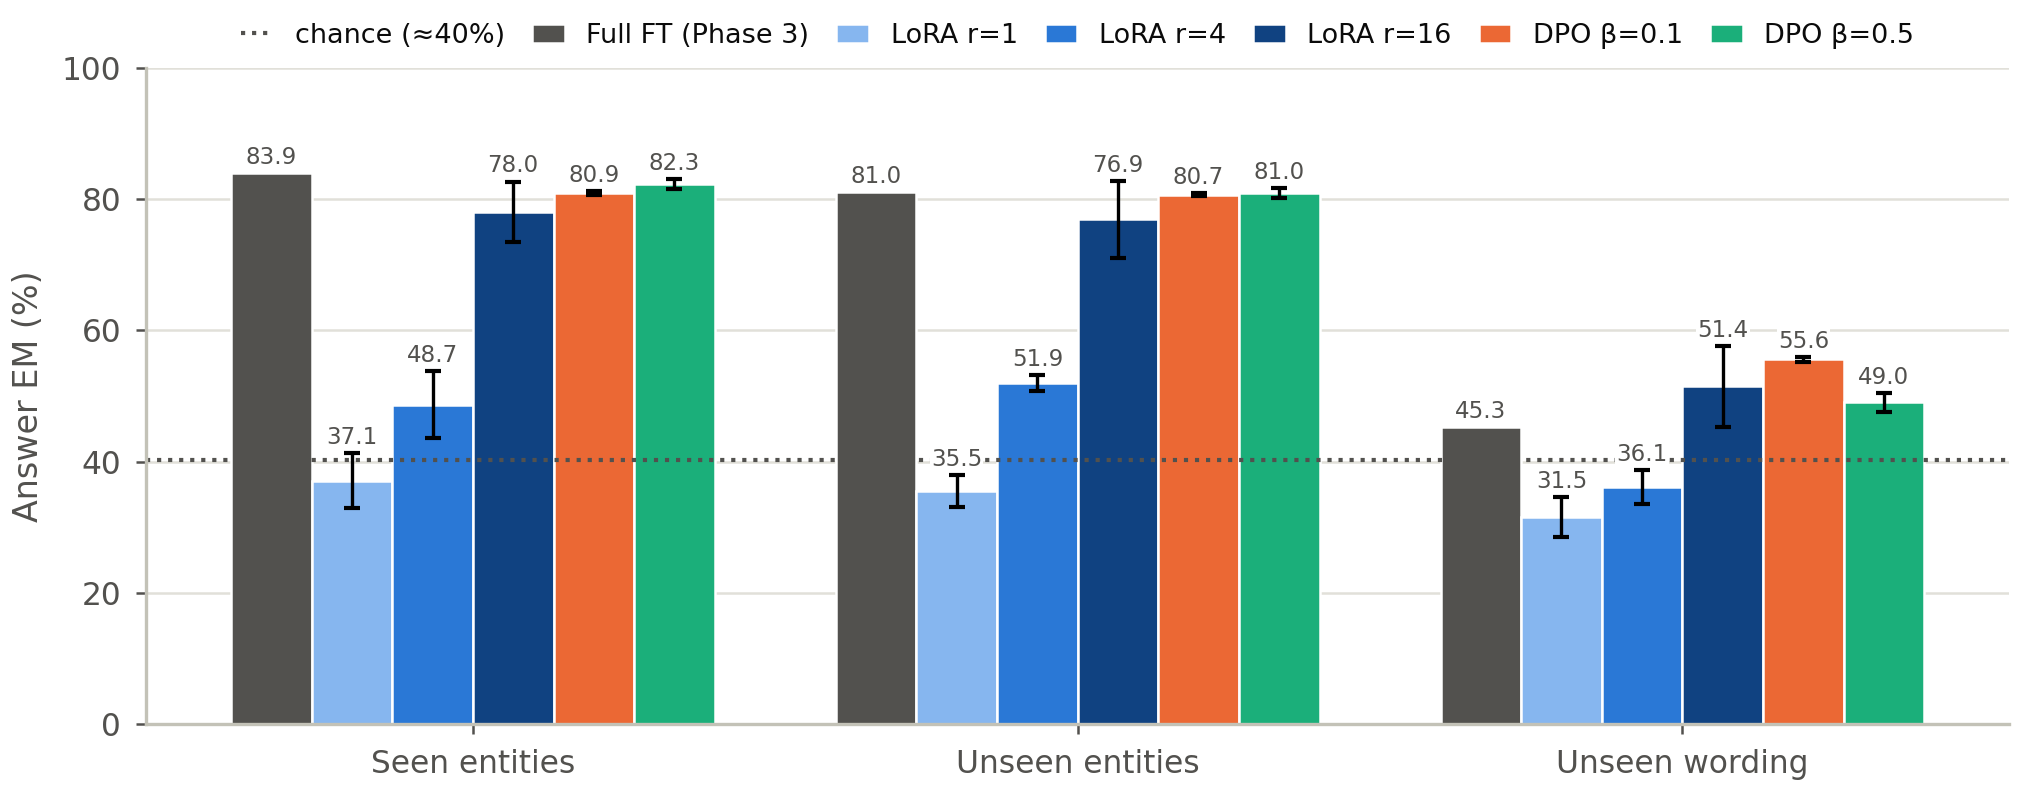
\includegraphics[width=\textwidth]{../figures/fig_ada_main.png}
\caption{A2/A4: answer EM on the three test sets. Full FT: the Phase 3 checkpoint; LoRA and DPO (chosen configuration): mean $\pm$ sd over 3 seeds. Dotted line: chance.}
\label{fig:sweep}
\end{figure}

\begin{figure}[H]
\centering
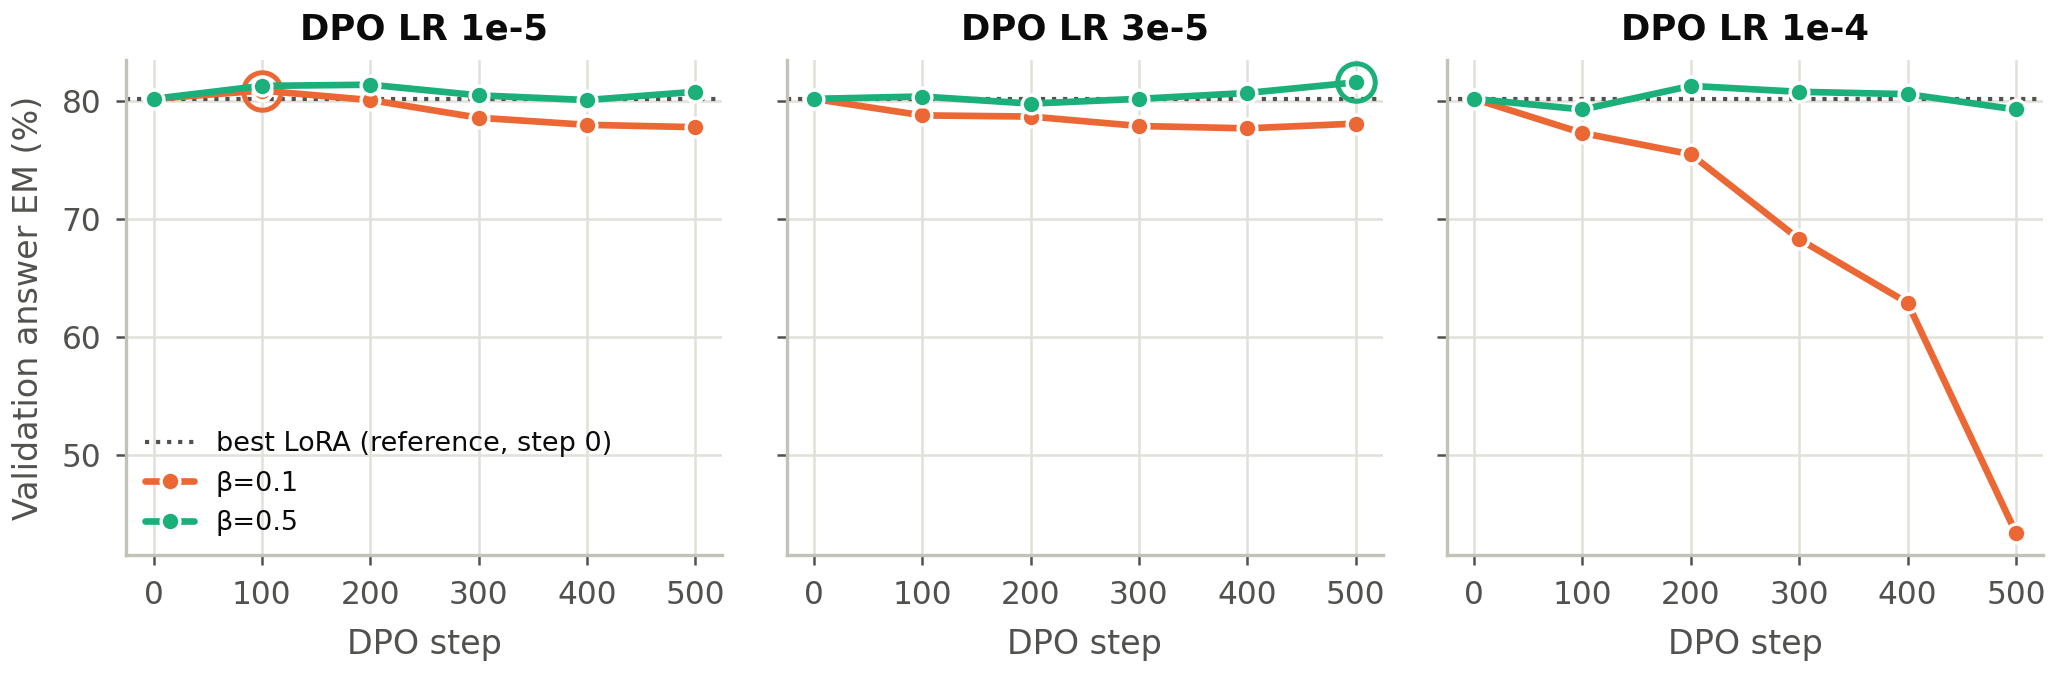
\includegraphics[width=\textwidth]{../figures/fig_a4_dpo_sweep_val.png}
\caption{A4: DPO sweep (seed 42). Validation answer EM of the policy saved every 100 steps, for each LR and both $\beta$; step 0 is the best LoRA model (dotted); the ring marks the configuration chosen for each $\beta$.}
\label{fig:dposweep}
\end{figure}

\begin{figure}[H]
\centering
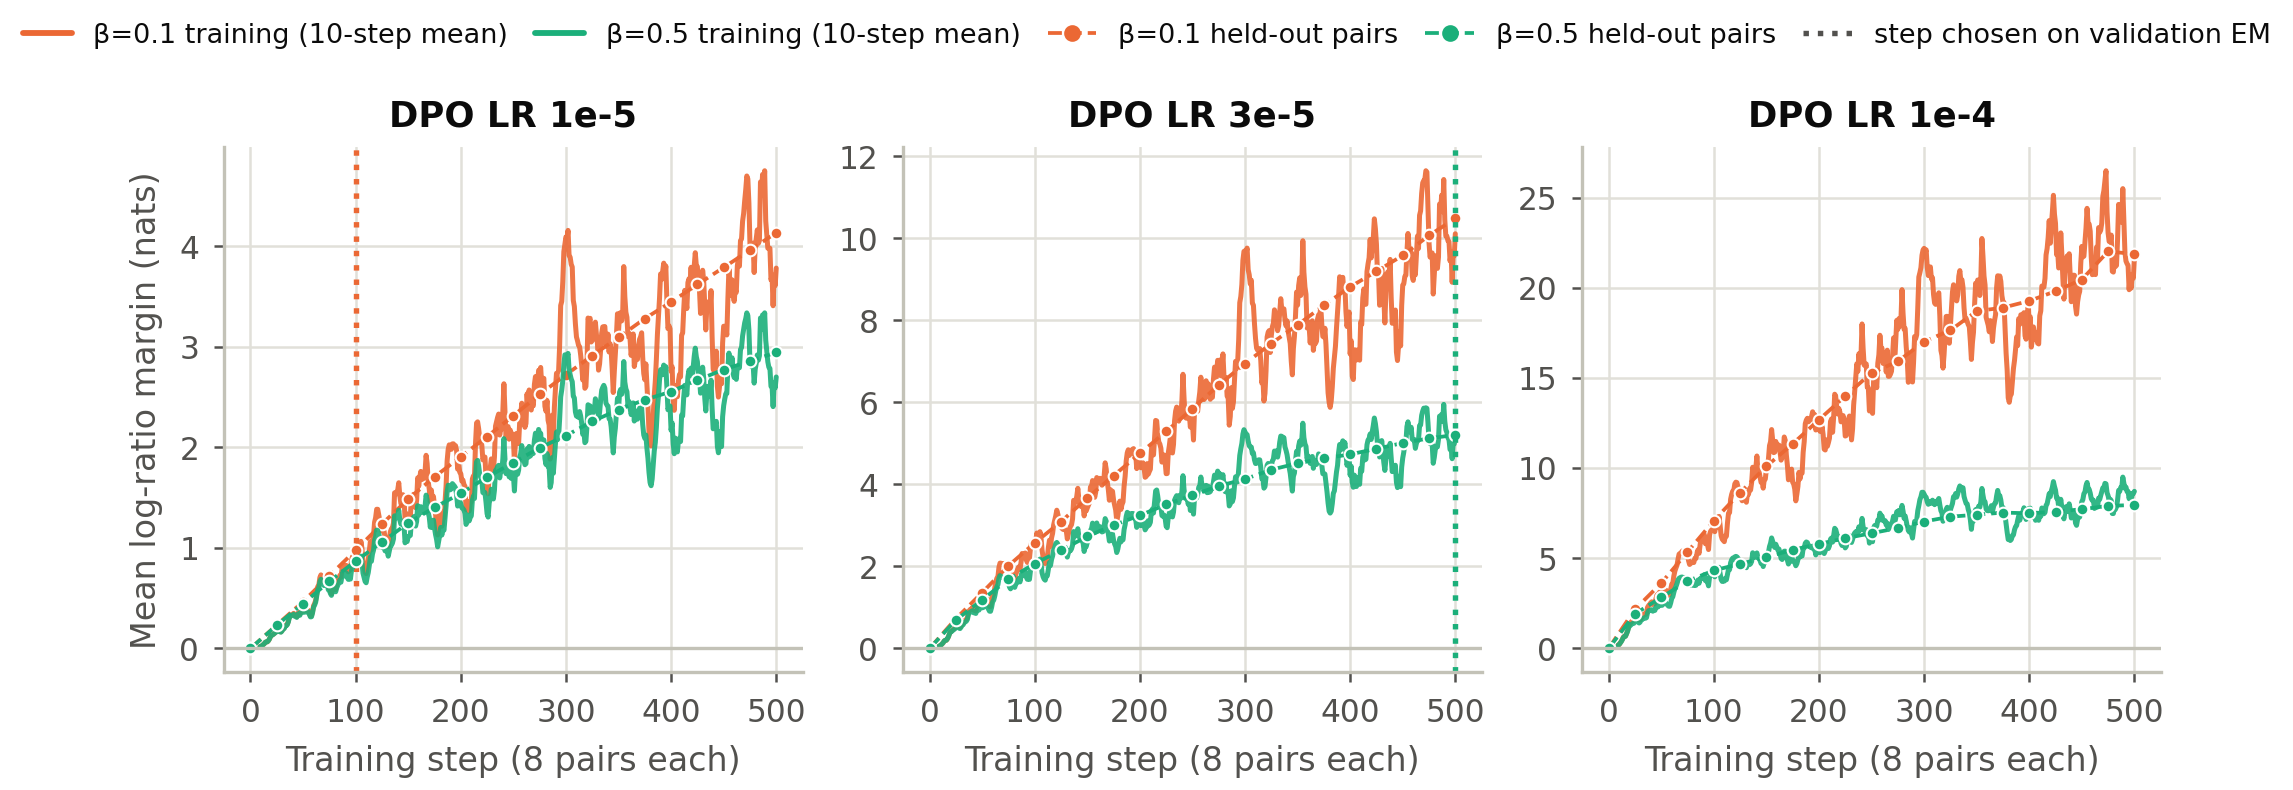
\includegraphics[width=\textwidth]{../figures/fig_ada_dpo_margins.png}
\caption{A4: mean chosen-minus-rejected log-ratio margin over DPO training for $\beta=0.1$ and $\beta=0.5$, at each LR (seed 42). Solid: training batches (10-step mean); dashed: the 400 held-out validation pairs; dotted vertical: the step chosen on validation accuracy.}
\label{fig:dpo}
\end{figure}

\begin{figure}[H]
\centering
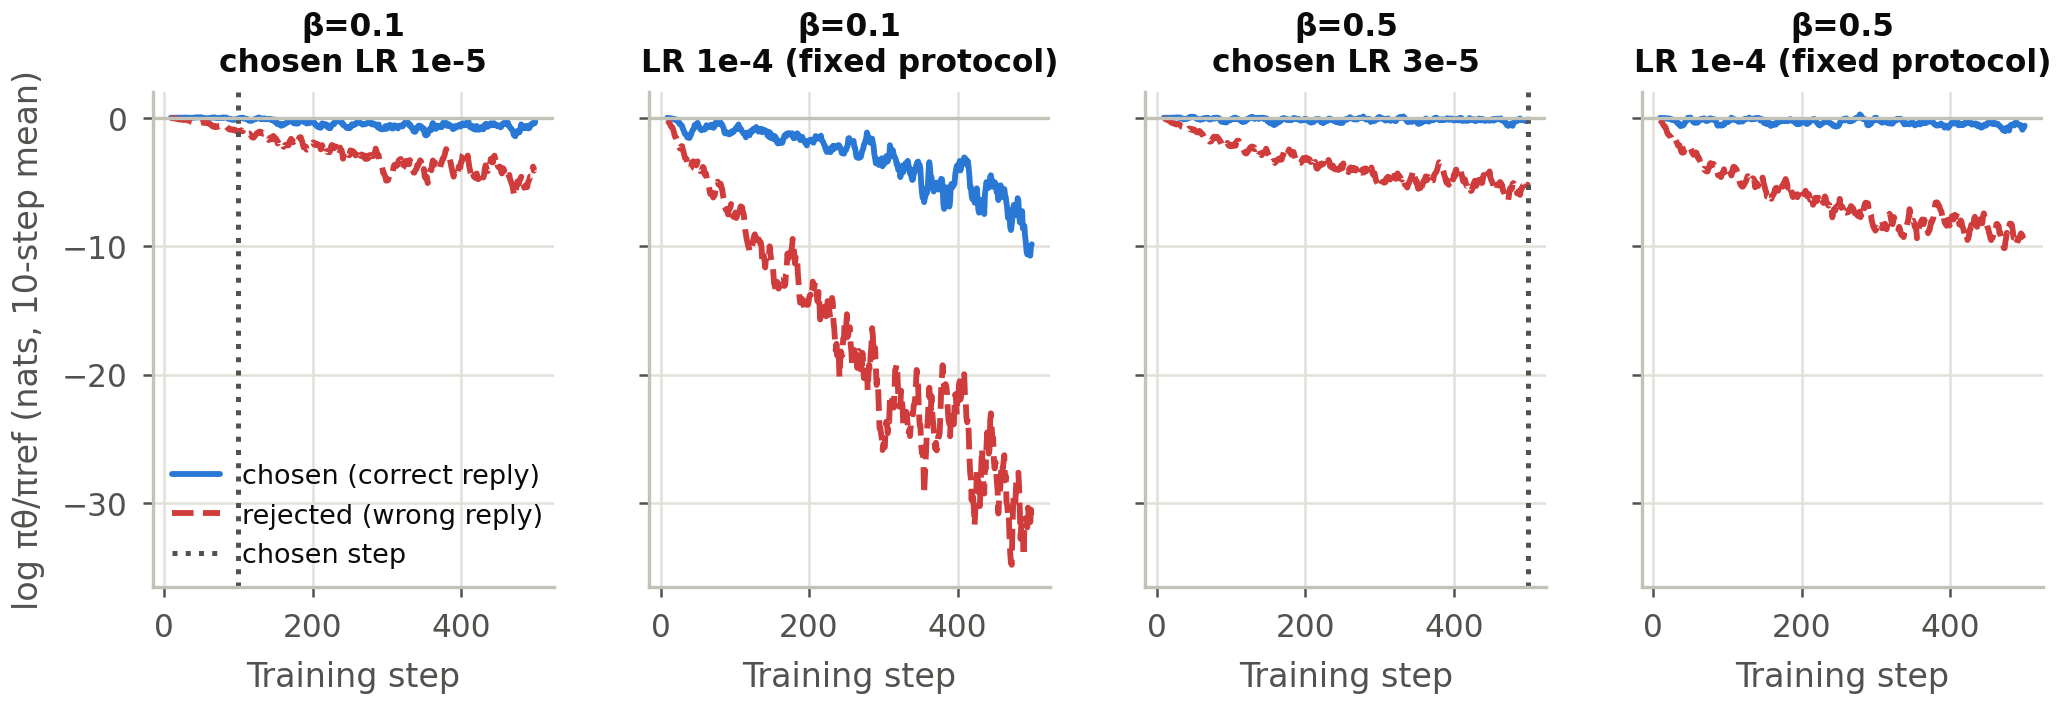
\includegraphics[width=\textwidth]{../figures/fig_ada_dpo_logratios.png}
\caption{A4: log-ratios $\log\pi_\theta/\pi_{\rm ref}$ of the chosen (correct) and the rejected (wrong) replies separately (seed 42), for each $\beta$'s chosen LR and for the fixed protocol (LR $10^{-4}$).}
\label{fig:logratios}
\end{figure}

\begin{figure}[H]
\centering
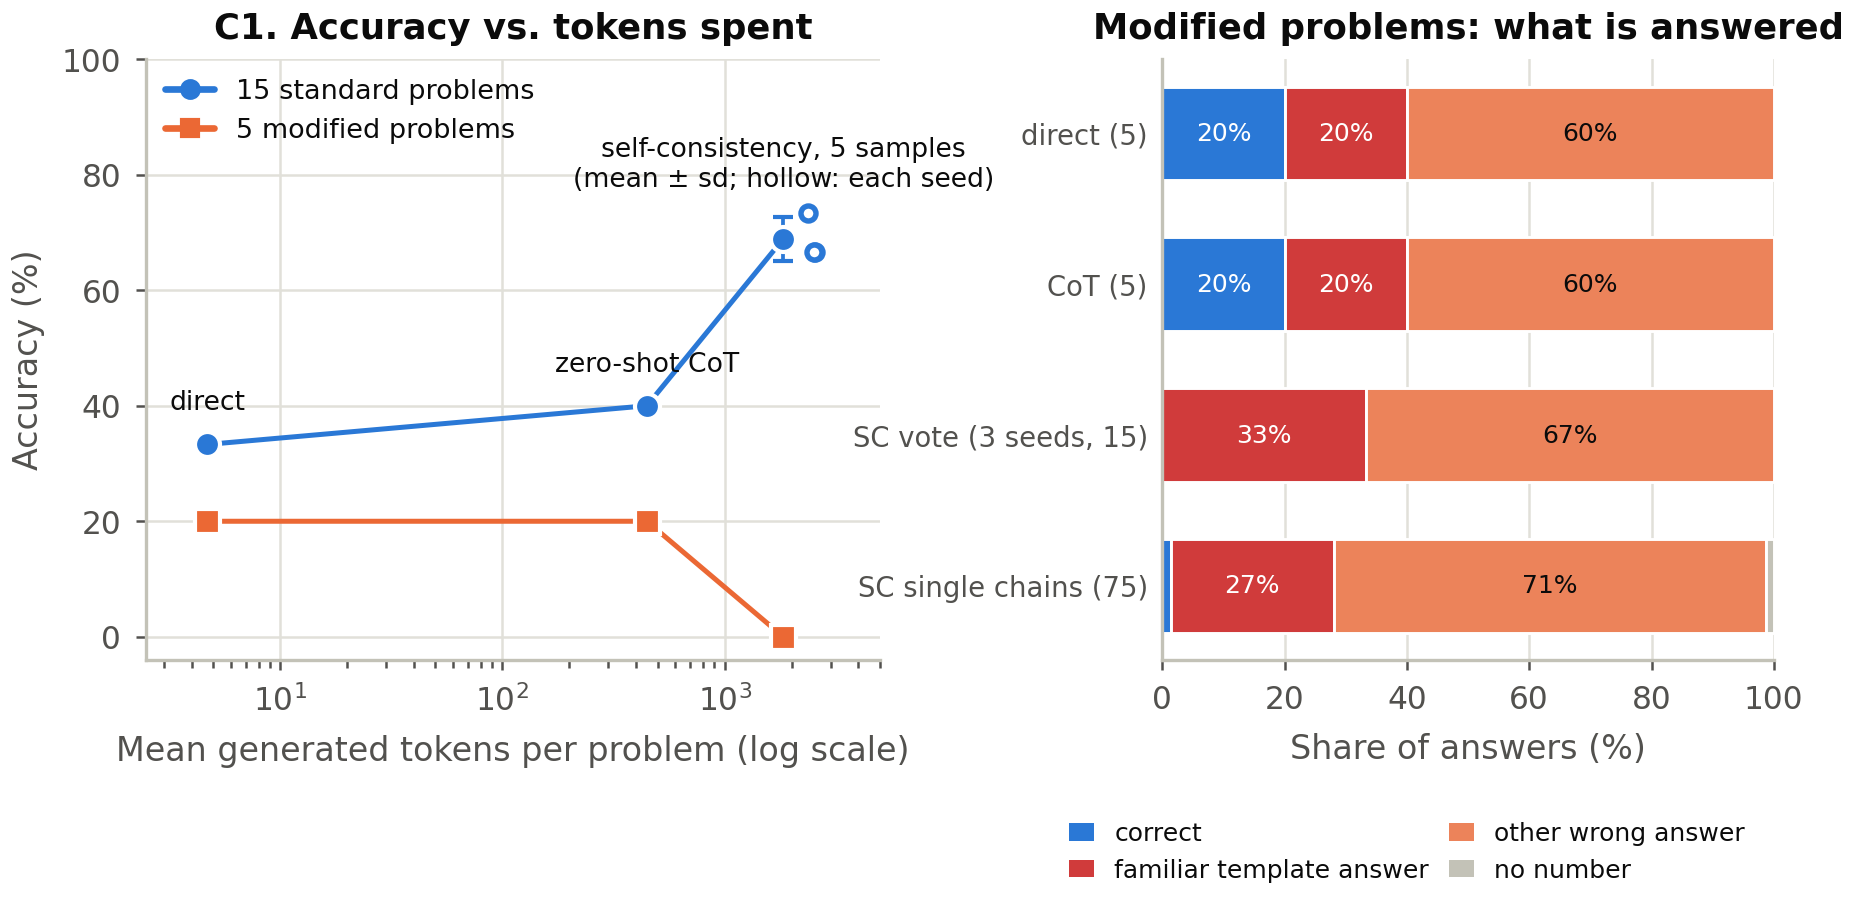
\includegraphics[width=\textwidth]{../figures/fig_eval_c1_tokens.png}
\caption{C1. \emph{Left:} accuracy against mean generated tokens per problem (log scale). Thinking longer helps on the 15 standard problems but not on the 5 modified ones: direct and CoT each solve one (M02 and M05), voting none. \emph{Right:} what the model answers on the modified problems: mostly another wrong number, and the familiar template's answer in a fifth to a third of the answers (such as 8 for ``all except 9''). One of the 75 sampled chains is right (M05); no vote is.}
\label{fig:c1tokens}
\end{figure}

\begin{figure}[H]
\centering
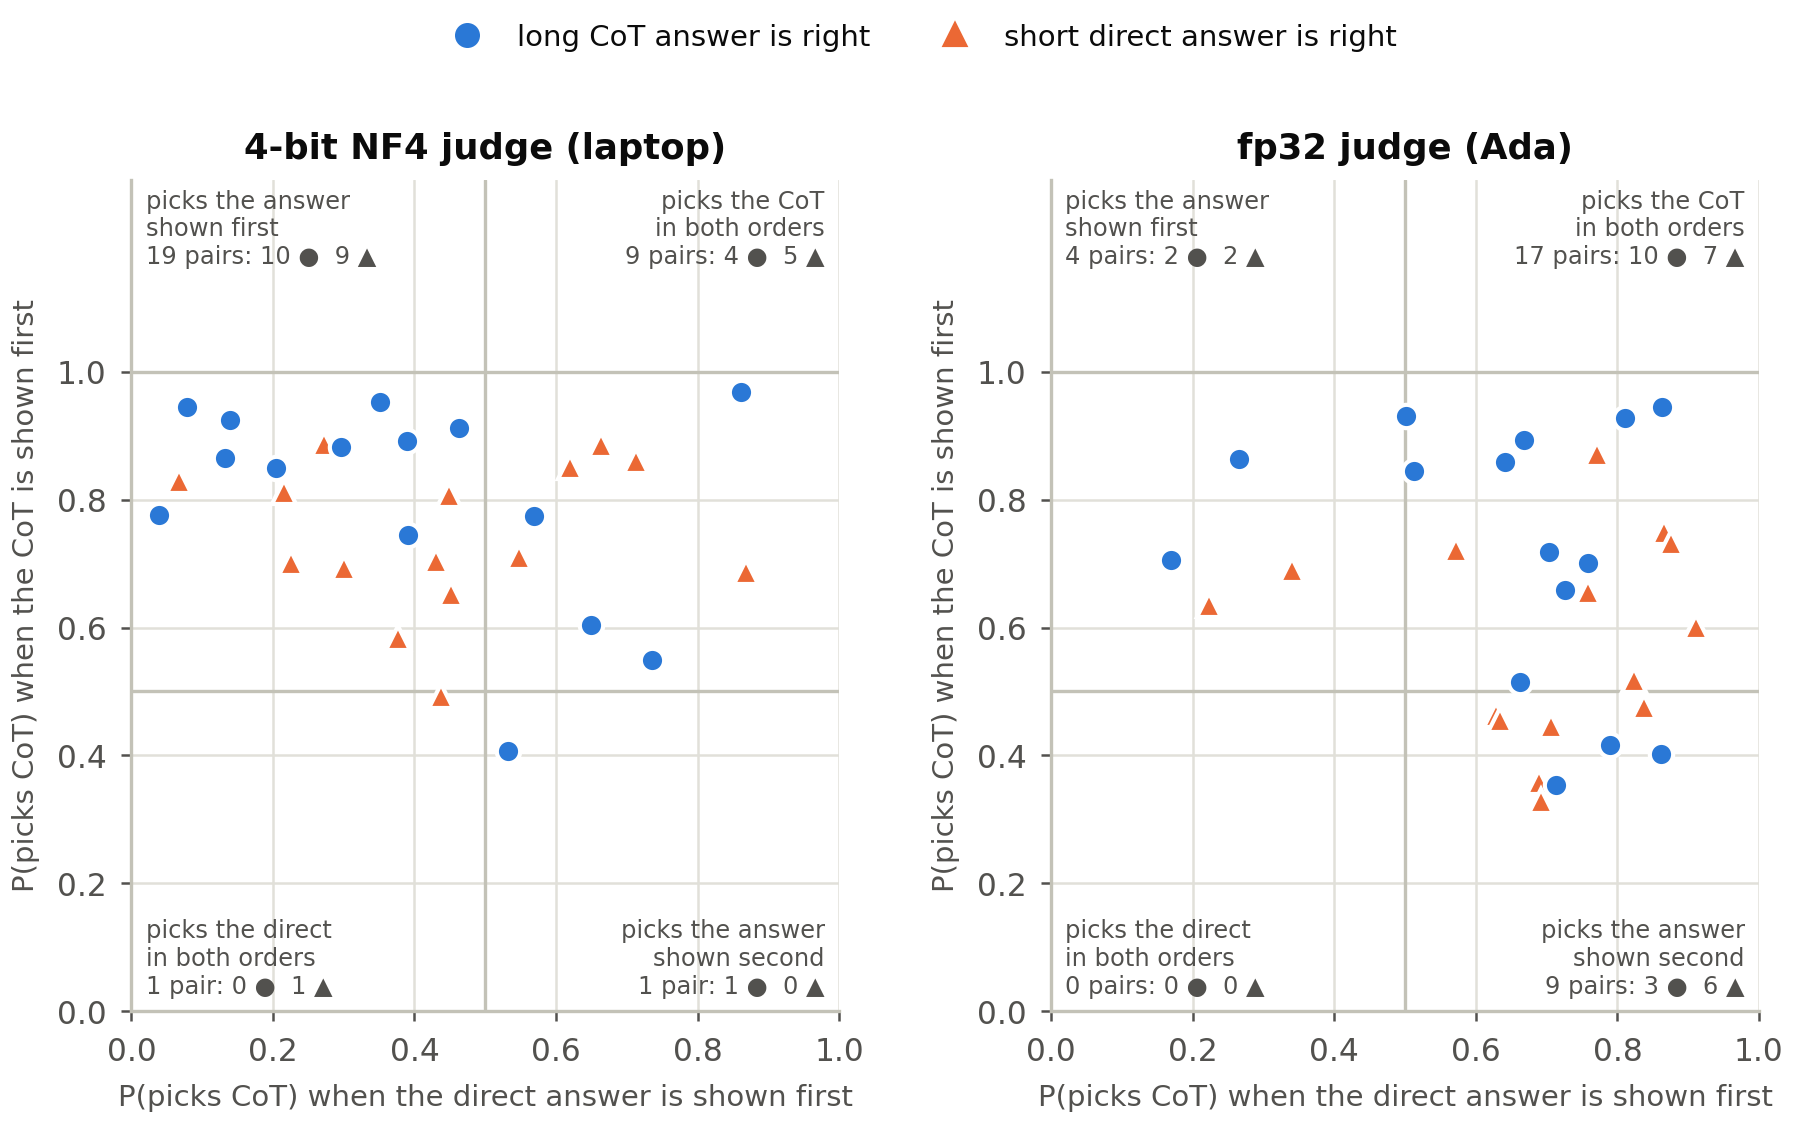
\includegraphics[width=\textwidth]{../figures/fig_eval_c2_judge.png}
\caption{C2: each of the 30 pairs, placed by the judge's probability of preferring the CoT reply when the direct reply is shown first ($x$) and when the CoT reply is shown first ($y$). The top-left and bottom-right quadrants are order flips. Counts: \textbullet\ pairs where the CoT reply is right, $\blacktriangle$ pairs where the direct reply is right. The 4-bit judge sits mostly top-left (it picks the first answer shown; \CTwoPosBiasN\ of 30 pairs flip). The fp32 judge sits mostly top-right (it picks the long CoT in both orders in \FpConsistent\ pairs, right or not; \FpPosBiasN\ flip). A judge that read for correctness would put \textbullet\ top-right and $\blacktriangle$ bottom-left.}
\label{fig:c2judge}
\end{figure}


\clearpage
\appendix
\raggedbottom
\section*{Appendix}

Commands to reproduce every number: \texttt{README.md} of the repository.

\subsection*{Held-out wording used by the unseen-wording test set}
{\small
\begin{tabular}{ll}
\toprule
Training frame (Phase 3 generator) & Held-out frame (\texttt{UnseenWordingHindi}) \\
\midrule
\dn{A, B और C तीन दोस्त हैं।} & \dn{A, B और C के बारे में कुछ जानकारी दी गई है।}\\
\dn{A की लंबाई B से अधिक है।} & \dn{A की लंबाई B की लंबाई से ज़्यादा है।}\\
\dn{B की लंबाई A से कम है।} & \dn{B की लंबाई A के मुकाबले कम है।}\\
\dn{B की तुलना में A की लंबाई अधिक है।} & \dn{A के मुकाबले B की लंबाई कम है।}\\
\dn{A B से लंबा है। / B A से छोटा है।} & \dn{A कद में B से लंबा है।}, \dn{A उम्र में B से बड़ा है।}, \dn{A वज़न में B से भारी है।}, \dn{A B से तेज़ दौड़ता है।}\\
\dn{A की लंबाई 150 सेमी है।} & \dn{A 150 सेमी लंबा है।}, \dn{A 25 वर्ष का है।}, \dn{A का भार 60 किग्रा है।}, \dn{A की कीमत 250 रुपये है।}\\
\dn{इनमें से किसकी लंबाई सबसे अधिक है?} & \dn{बताइए, सबसे ज़्यादा लंबाई किसकी है?}\\
\dn{क्या A की लंबाई B से अधिक है?} & \dn{क्या यह सही है कि A की लंबाई B से ज़्यादा है?}\\
\dn{A और B में से किसकी लंबाई अधिक है?} & \dn{A या B, किसकी लंबाई ज़्यादा है?}\\
\dn{क्या A और B की लंबाई बराबर है?} & \dn{क्या A की लंबाई और B की लंबाई समान है?}\\
\bottomrule
\end{tabular}}

\subsection*{Part C prompts (verbatim user-turn suffixes; Qwen's default system prompt)}
Direct: ``\dn{केवल अंतिम उत्तर एक संख्या के रूप में लिखिए। कोई व्याख्या या इकाई मत लिखिए।}''\\
CoT and self-consistency: ``\dn{आइए चरण-दर-चरण सोचें। अपना हल लिखिए और अंत में 'उत्तर: <संख्या>' लिखिए।}''\\
Judge (system): ``You are an impartial judge who checks solutions to math word problems.'' Judge (user): ``Below is a math word problem written in Hindi, followed by two candidate answers. Problem: \ldots\ Answer A: \ldots\ Answer B: \ldots\ Which answer is better, that is, more likely to reach the correct final result? Reply with only one letter: A or B.''

\subsection*{First pass (laptop, seed 42, LR $10^{-3}$ for every rank): answer EM \% (chain EM)}
\begin{tabular}{lcccc}\toprule model & val & seen ent. & unseen ent. & unseen word.\\\midrule
Full FT (Phase 3) & 82.9 (74.5) & 83.9 (81.6) & 81.0 (72.9) & 45.3 (3.1)\\
LoRA r=1 & 36.0 (3.1) & 32.2 (2.5) & 36.4 (2.8) & 31.3 (1.0)\\
LoRA r=4 & 54.1 (39.5) & 60.9 (45.9) & 55.8 (40.8) & 44.3 (7.4)\\
LoRA r=16 & 65.6 (54.8) & 63.5 (56.0) & 63.1 (53.5) & 45.3 (5.5)\\
DPO $\beta$=0.1 (LR 1e-4, 500 steps) & 35.4 (23.8) & 39.4 (28.6) & 31.9 (22.3) & 32.5 (1.9)\\
DPO $\beta$=0.5 (LR 1e-4, 500 steps) & 63.0 (53.0) & 69.4 (62.2) & 62.4 (52.0) & 42.8 (5.0)\\
\bottomrule\end{tabular}

\subsection*{A3: one preference pair per question type (prompt abridged to the question)}
\begin{footnotesize}
\textbf{numeric\_pair\_yesno} (the two numbers compared the wrong way round).\\
\dn{प्रश्न}: \dn{रज़ाई और झाड़ू दो वस्तुएँ हैं। झाड़ू का मूल्य }302 \dn{रुपये है। रज़ाई का मूल्य }884 \dn{रुपये है। क्या झाड़ू का मूल्य रज़ाई से अधिक है}?\\
\textit{chosen:} 302 = \dn{झाड़ू और }884 = \dn{रज़ाई है। }302 \textless{} 884 \dn{है}, \dn{अतः झाड़ू }\textless{} \dn{रज़ाई है। प्रश्न का दावा झाड़ू }\textgreater{} \dn{रज़ाई है।}
\dn{उत्तर}: \dn{नहीं}\\
\textit{rejected:} 302 = \dn{झाड़ू और }884 = \dn{रज़ाई है। }302 \textgreater{} 884 \dn{है}, \dn{अतः झाड़ू }\textgreater{} \dn{रज़ाई है। प्रश्न का दावा झाड़ू }\textgreater{} \dn{रज़ाई है।}
\dn{उत्तर}: \dn{हाँ}\\[3pt]
\textbf{transitive\_max} (order built with the two extreme-end entities swapped).\\
\dn{प्रश्न}: \dn{अर्जुन}, \dn{जयंत}, \dn{मिथुन और मोहिनी चार दोस्त हैं। जयंत की लंबाई अर्जुन से अधिक है। मिथुन जयंत से लंबा है। मिथुन मोहिनी से छोटा है। इनमें से किसकी लंबाई सबसे अधिक है}?\\
\textit{chosen:} \dn{जयंत }\textgreater{} \dn{अर्जुन और मिथुन }\textgreater{} \dn{जयंत और मिथुन }\textless{} \dn{मोहिनी है। अर्थात् जयंत }\textgreater{} \dn{अर्जुन और मिथुन }\textgreater{} \dn{जयंत और मोहिनी }\textgreater{} \dn{मिथुन है। क्रम}: \dn{मोहिनी }\textgreater{} \dn{मिथुन }\textgreater{} \dn{जयंत }\textgreater{} \dn{अर्जुन है। अतः सबसे अधिक लंबाई मोहिनी की है।}
\dn{उत्तर}: \dn{मोहिनी}\\
\textit{rejected:} \dn{जयंत }\textgreater{} \dn{अर्जुन और मिथुन }\textgreater{} \dn{जयंत और मिथुन }\textless{} \dn{मोहिनी है। अर्थात् जयंत }\textgreater{} \dn{अर्जुन और मिथुन }\textgreater{} \dn{जयंत और मोहिनी }\textgreater{} \dn{मिथुन है। क्रम}: \dn{मिथुन }\textgreater{} \dn{मोहिनी }\textgreater{} \dn{जयंत }\textgreater{} \dn{अर्जुन है। अतः सबसे अधिक लंबाई मिथुन की है।}
\dn{उत्तर}: \dn{मिथुन}\\[3pt]
\textbf{numeric\_pair\_which} (the two numbers compared the wrong way round).\\
\dn{प्रश्न}: \dn{मोहिनी और वंदना दो दोस्त हैं। वंदना की आयु }84 \dn{वर्ष है। मोहिनी की आयु }55 \dn{वर्ष है। मोहिनी और वंदना में से किसकी आयु कम है}?\\
\textit{chosen:} 84 = \dn{वंदना और }55 = \dn{मोहिनी है। }84 \textgreater{} 55 \dn{है}, \dn{अतः वंदना }\textgreater{} \dn{मोहिनी है।}
\dn{उत्तर}: \dn{मोहिनी}\\
\textit{rejected:} 84 = \dn{वंदना और }55 = \dn{मोहिनी है। }84 \textless{} 55 \dn{है}, \dn{अतः मोहिनी }\textgreater{} \dn{वंदना है।}
\dn{उत्तर}: \dn{वंदना}\\[3pt]
\textbf{verbal\_yesno} (asked relation derived the wrong way round).\\
\dn{प्रश्न}: \dn{सलोनी और सोनाली दो दोस्त हैं। सलोनी सोनाली से हल्की है। क्या सोनाली का वजन सलोनी से कम है}?\\
\textit{chosen:} \dn{कथन के अनुसार सलोनी }\textless{} \dn{सोनाली है}, \dn{अतः सोनाली }\textgreater{} \dn{सलोनी है। प्रश्न का दावा सोनाली }\textless{} \dn{सलोनी है।}
\dn{उत्तर}: \dn{नहीं}\\
\textit{rejected:} \dn{कथन के अनुसार सलोनी }\textless{} \dn{सोनाली है}, \dn{अतः सोनाली }\textless{} \dn{सलोनी है। प्रश्न का दावा सोनाली }\textless{} \dn{सलोनी है।}
\dn{उत्तर}: \dn{हाँ}\\[3pt]
\textbf{numeric\_extremum\_min} (runner-up value picked as the extreme).\\
\dn{प्रश्न}: \dn{चटाई}, \dn{कीबोर्ड और रबर तीन वस्तुएँ हैं। चटाई का मूल्य }221 \dn{रुपये है। रबर का मूल्य }95 \dn{रुपये है। कीबोर्ड का मूल्य }165 \dn{रुपये है। इनमें से किस वस्तु का मूल्य सबसे कम है}?\\
\textit{chosen:} 221 = \dn{चटाई और }95 = \dn{रबर और }165 = \dn{कीबोर्ड है। सबसे कम मान }95 = \dn{रबर है।}
\dn{उत्तर}: \dn{रबर}\\
\textit{rejected:} 221 = \dn{चटाई और }95 = \dn{रबर और }165 = \dn{कीबोर्ड है। सबसे कम मान }165 = \dn{कीबोर्ड है।}
\dn{उत्तर}: \dn{कीबोर्ड}\\[3pt]
\textbf{transitive\_min} (order built with the two extreme-end entities swapped).\\
\dn{प्रश्न}: \dn{प्रतिभा}, \dn{साधना और कृष्ण तीन दोस्त हैं। प्रतिभा साधना से भारी है। साधना का वजन कृष्ण से अधिक है। इनमें से किसका वजन सबसे कम है}?\\
\textit{chosen:} \dn{प्रतिभा }\textgreater{} \dn{साधना और साधना }\textgreater{} \dn{कृष्ण है। अर्थात् प्रतिभा }\textgreater{} \dn{साधना और साधना }\textgreater{} \dn{कृष्ण है। क्रम}: \dn{प्रतिभा }\textgreater{} \dn{साधना }\textgreater{} \dn{कृष्ण है। अतः सबसे कम वजन कृष्ण का है।}
\dn{उत्तर}: \dn{कृष्ण}\\
\textit{rejected:} \dn{प्रतिभा }\textgreater{} \dn{साधना और साधना }\textgreater{} \dn{कृष्ण है। अर्थात् प्रतिभा }\textgreater{} \dn{साधना और साधना }\textgreater{} \dn{कृष्ण है। क्रम}: \dn{प्रतिभा }\textgreater{} \dn{कृष्ण }\textgreater{} \dn{साधना है। अतः सबसे कम वजन साधना का है।}
\dn{उत्तर}: \dn{साधना}\\[3pt]
\textbf{transitive\_yesno} (relation of the asked pair read backwards from the order).\\
\dn{प्रश्न}: \dn{रमेश}, \dn{योगेश}, \dn{पल्लवी और वंदना चार दोस्त हैं। योगेश वंदना से छोटा है। रमेश पल्लवी से छोटा है। रमेश वंदना से बड़ा है। क्या पल्लवी की आयु योगेश से अधिक है}?\\
\textit{chosen:} \dn{योगेश }\textless{} \dn{वंदना और रमेश }\textless{} \dn{पल्लवी और रमेश }\textgreater{} \dn{वंदना है। अर्थात् वंदना }\textgreater{} \dn{योगेश और पल्लवी }\textgreater{} \dn{रमेश और रमेश }\textgreater{} \dn{वंदना है। क्रम}: \dn{पल्लवी }\textgreater{} \dn{रमेश }\textgreater{} \dn{वंदना }\textgreater{} \dn{योगेश है। अतः पल्लवी }\textgreater{} \dn{योगेश है। प्रश्न का दावा पल्लवी }\textgreater{} \dn{योगेश है।}
\dn{उत्तर}: \dn{हाँ}\\
\textit{rejected:} \dn{योगेश }\textless{} \dn{वंदना और रमेश }\textless{} \dn{पल्लवी और रमेश }\textgreater{} \dn{वंदना है। अर्थात् वंदना }\textgreater{} \dn{योगेश और पल्लवी }\textgreater{} \dn{रमेश और रमेश }\textgreater{} \dn{वंदना है। क्रम}: \dn{पल्लवी }\textgreater{} \dn{रमेश }\textgreater{} \dn{वंदना }\textgreater{} \dn{योगेश है। अतः पल्लवी }\textless{} \dn{योगेश है। प्रश्न का दावा पल्लवी }\textgreater{} \dn{योगेश है।}
\dn{उत्तर}: \dn{नहीं}\\[3pt]
\textbf{numeric\_extremum\_max} (runner-up value picked as the extreme).\\
\dn{प्रश्न}: \dn{वसुधा}, \dn{हिना और अनिल तीन दोस्त हैं। वसुधा की लंबाई }193 \dn{सेमी है। हिना की लंबाई }131 \dn{सेमी है। अनिल की लंबाई }157 \dn{सेमी है। इनमें से किसकी लंबाई सबसे अधिक है}?\\
\textit{chosen:} 193 = \dn{वसुधा और }131 = \dn{हिना और }157 = \dn{अनिल है। सबसे अधिक मान }193 = \dn{वसुधा है।}
\dn{उत्तर}: \dn{वसुधा}\\
\textit{rejected:} 193 = \dn{वसुधा और }131 = \dn{हिना और }157 = \dn{अनिल है। सबसे अधिक मान }157 = \dn{अनिल है।}
\dn{उत्तर}: \dn{अनिल}\\[3pt]
\end{footnotesize}

\subsection*{Ada study: LoRA learning-rate grid (seed 42, 5 epochs; choice = lowest validation loss per rank)}
\begin{tabular}{llcccc}\toprule rank & LR & best val.\ loss (epoch) & val.\ EM & unseen-entity EM & chosen\\\midrule
$r=1$ & 3e-4 & 0.5045 (5) & 37.8 & 37.3 & \checkmark\\
$r=1$ & 1e-3 & 0.5145 (5) & 38.0 & 36.5 & \\
$r=1$ & 3e-3 & 0.6940 (5) & 32.4 & 33.7 & \\
$r=4$ & 3e-4 & 0.1778 (5) & 42.1 & 47.5 & \\
$r=4$ & 1e-3 & 0.1627 (5) & 48.7 & 51.0 & \checkmark\\
$r=4$ & 3e-3 & 0.2397 (4) & 43.5 & 46.1 & \\
$r=16$ & 3e-4 & 0.0882 (5) & 60.4 & 60.7 & \\
$r=16$ & 1e-3 & 0.0785 (5) & 73.4 & 70.2 & \checkmark\\
$r=16$ & 3e-3 & 0.1232 (4) & 69.5 & 67.4 & \\
\bottomrule\end{tabular}

\subsection*{Ada study: DPO sweep, validation answer EM (\%) of the policy saved every 100 steps (seed 42; step 0 = best LoRA, 80.2)}
\begin{tabular}{llccccccc}\toprule $\beta$ & LR & 100 & 200 & 300 & 400 & 500 & val.\ margin (500) & pref.\ acc.\\\midrule
0.1 & 1e-5 & \textbf{80.9} & 80.1 & 78.6 & 78.0 & 77.8 & 4.1 & 83.5\%\\
0.1 & 3e-5 & 78.8 & 78.7 & 77.9 & 77.7 & 78.1 & 10.5 & 87.8\%\\
0.1 & 1e-4 & 77.3 & 75.5 & 68.3 & 62.9 & 43.4 & 21.9 & 86.8\%\\
0.5 & 1e-5 & 81.3 & 81.4 & 80.5 & 80.1 & 80.8 & 2.9 & 86.5\%\\
0.5 & 3e-5 & 80.4 & 79.8 & 80.2 & 80.7 & \textbf{81.6} & 5.2 & 89.5\%\\
0.5 & 1e-4 & 79.3 & 81.3 & 80.8 & 80.6 & 79.3 & 8.0 & 88.0\%\\
\bottomrule\end{tabular}

Bold: the configuration chosen for each $\beta$ (highest validation EM; ties go to fewer steps).



\subsection*{Notes and limitations}
\begin{itemize}[leftmargin=*,nosep]
\item The Phase 3 project had a single (unseen-entity) test set. The seen-entity and unseen-wording sets were built for this assignment with the project generator, and the Phase 3 full-finetune checkpoint was re-scored on them, so every row of Table~\ref{tab:sweep} uses the same three sets.
\item Two passes. The first, single-seed pass ran on the laptop (RTX 4050). The tables come from the Ada study (3 seeds, per-rank LR, DPO LR and step chosen on validation). Scoring the same checkpoint gives identical numbers on both GPUs (last row of the cross-check table), but \emph{training} the same configuration and seed gives different models: floating-point differences change the training trajectory. This is why single-run differences of a few points are not interpreted, and why the main tables report mean$\pm$sd over seeds.
\item C2 pairs need exactly one correct reply, so ``short answer right'' pairs can only come from the problems where Qwen's direct answer is right (\CTwoShortRightProblems). The larger CoT pool (16 chains per problem) lets every one of them contribute.
\item C1: S14's chain answers ``2:30'' (2 h 30 min) to a question asking for minutes. The strict checker marks it wrong; a lenient grader might accept it. No other score depends on such a judgement call.
\item The modified problem M01 is the class's drifting-boat example (engine 15\,km/h in still water, current 3\,km/h, 8\,h drifting from A to B; how long back?) set on S01's boat (12\,km/h, current 3\,km/h, 6\,h): the answer is 2\,h, the template 10\,h.
\end{itemize}

\subsection*{Note}
Claude Code was used to help with coding help in the assignment.

\end{document}
